% Options for packages loaded elsewhere
\PassOptionsToPackage{unicode}{hyperref}
\PassOptionsToPackage{hyphens}{url}
\PassOptionsToPackage{space}{xeCJK}
%
\documentclass[
  11pt,
  letterpaper,
]{article}
\usepackage{amsmath,amssymb}
\usepackage{iftex}
\ifPDFTeX
  \usepackage[T1]{fontenc}
  \usepackage[utf8]{inputenc}
  \usepackage{textcomp} % provide euro and other symbols
\else % if luatex or xetex
  \usepackage{unicode-math} % this also loads fontspec
  \defaultfontfeatures{Scale=MatchLowercase}
  \defaultfontfeatures[\rmfamily]{Ligatures=TeX,Scale=1}
\fi
\usepackage{lmodern}
\ifPDFTeX\else
  % xetex/luatex font selection
  \ifXeTeX
    \usepackage{xeCJK}
    \setCJKmainfont[]{Noto Sans CJK SC}
          \fi
  \ifLuaTeX
    \usepackage[]{luatexja-fontspec}
    \setmainjfont[]{Noto Sans CJK SC}
  \fi
\fi
% Use upquote if available, for straight quotes in verbatim environments
\IfFileExists{upquote.sty}{\usepackage{upquote}}{}
\IfFileExists{microtype.sty}{% use microtype if available
  \usepackage[]{microtype}
  \UseMicrotypeSet[protrusion]{basicmath} % disable protrusion for tt fonts
}{}
\makeatletter
\@ifundefined{KOMAClassName}{% if non-KOMA class
  \IfFileExists{parskip.sty}{%
    \usepackage{parskip}
  }{% else
    \setlength{\parindent}{0pt}
    \setlength{\parskip}{6pt plus 2pt minus 1pt}}
}{% if KOMA class
  \KOMAoptions{parskip=half}}
\makeatother
\usepackage{xcolor}
\usepackage[margin=0.75in]{geometry}
\usepackage{graphicx}
\makeatletter
\def\maxwidth{\ifdim\Gin@nat@width>\linewidth\linewidth\else\Gin@nat@width\fi}
\def\maxheight{\ifdim\Gin@nat@height>\textheight\textheight\else\Gin@nat@height\fi}
\makeatother
% Scale images if necessary, so that they will not overflow the page
% margins by default, and it is still possible to overwrite the defaults
% using explicit options in \includegraphics[width, height, ...]{}
\setkeys{Gin}{width=\maxwidth,height=\maxheight,keepaspectratio}
% Set default figure placement to htbp
\makeatletter
\def\fps@figure{htbp}
\makeatother
\setlength{\emergencystretch}{3em} % prevent overfull lines
\providecommand{\tightlist}{%
  \setlength{\itemsep}{0pt}\setlength{\parskip}{0pt}}
\setcounter{secnumdepth}{-\maxdimen} % remove section numbering
\ifLuaTeX
  \usepackage{selnolig}  % disable illegal ligatures
\fi
\usepackage{bookmark}
\IfFileExists{xurl.sty}{\usepackage{xurl}}{} % add URL line breaks if available
\urlstyle{same}
\hypersetup{
  hidelinks,
  pdfcreator={LaTeX via pandoc}}

% \setcounter{tocdepth}{4}    % Show up to paragraph level in TOC
% \setcounter{secnumdepth}{4} % Number up to paragraph level

\author{}
\date{}

\begin{document}

\section{A New Exploration into Chinese Characters: from Simplification
to Deeper
Understanding}\label{a-new-exploration-into-chinese-characters-from-simplification-to-deeper-understanding}

Wen G. Gong*

*Corresponding author: wen\_gong@vanguard.com

\subsection{Abstract}\label{abstract}

This paper presents a novel approach to Chinese characters through the
lens of physics, network analysis, and natural systems. Computational
analysis of over 6,000 characters identified 422 elemental characters
(元字) as fundamental building blocks. Using a physics-inspired
``Zi-Matrix'' model, we analyzed character structure across eleven
spatial positions, revealing systematic patterns in component
relationships and semantic extension.

Our research demonstrates that Chinese characters exhibit properties of
natural systems: emergent complexity, self-organization, and adaptive
resilience. The Fibonacci sequence provides an organizing framework for
understanding character evolution, from simple pictographs to
sophisticated abstractions. Case studies of character families and
semantic networks show how meaning radiates from concrete to abstract
domains while maintaining coherent principles.

By viewing Chinese characters as a living system, this research
transcends mere simplification to reveal how human cognition organizes
and transmits knowledge. While the elemental character set reduces
memorization burden, it also illuminates profound connections between
language, thought, and natural patterns. Chinese characters emerge not
just as tools for communication, but as windows into human
understanding. This perspective, combined with AI-assisted learning
approaches, promises to transform language education from knowledge
mastery to meaning discovery, bridging traditional wisdom with modern
computational methods.

Keywords: Chinese characters, network analysis, natural systems,
cognitive linguistics, computational linguistics, language learning,
knowledge organization

\subsection{Motivation}\label{motivation}

Learning 汉字 (Hànzì) and, by extension, the Chinese language presents a
unique and substantial challenge for learners, particularly those whose
native languages utilize alphabetic systems. The difficulty stems
primarily from the logographic nature of 汉字, where each character
represents a morpheme (or word) rather than a sound. Unlike phonetic
scripts, there's often no readily apparent connection between a
character's visual form and its pronunciation, demanding rote
memorization of thousands of distinct characters to achieve basic
literacy. This is compounded by the tonal nature of Mandarin Chinese,
where changes in pitch can drastically alter the meaning of a word,
adding another layer of complexity. Furthermore, the sheer volume of
characters, the subtle nuances in stroke order and character
composition, and the existence of both traditional and simplified forms,
require a sustained and dedicated learning effort over a prolonged
period, making the acquisition of fluency in written and spoken Chinese
a significantly time-intensive undertaking compared to many other
languages.

Inspired by the success of reductionism in science, such as the
discovery of fundamental particles in physics and the organization of
the periodic table in chemistry, this research seeks to apply similar
principles to the learning of 汉字. This involves three key approaches:

\begin{itemize}
\item
  \textbf{Network Analysis}: Leveraging computer science and network
  analysis techniques, this study aims to uncover the hidden
  relationships and underlying structures within the large collection of
  Chinese characters. By mapping these connections, the research hopes
  to reveal patterns and simplify the seemingly chaotic complexity of
  the character system.
\item
  \textbf{Artificial Intelligence (AI) Assistance}: Recognizing the
  burden of rote memorization in traditional 汉字 learning, this
  research explores the use of AI to alleviate this challenge. The goal
  is to develop AI-powered tools that can assist learners in memorizing
  the form, pronunciation, and meaning of characters, as well as their
  complex interactions and contextual usage.
\item
  \textbf{Improve learning and learning expeirence}: The overarching
  research goal, built upon by applying network analysis and AI
  asisstance, is to reduce the learning burdens for students and enrich
  their learning experiences.
\end{itemize}

By combining these computational and AI-driven approaches with a
reductionist perspective, the research aims to provide a novel
exploration into understanding and learning 汉字, ultimately making the
process more efficient, intuitive, and enjoyable for learners.

\subsection{Computational Network Analysis on Chinese
Characters}\label{computational-network-analysis-on-chinese-characters}

The foundational work Shuowen Jiezi (《说文解字》), compiled by Xu Shen
(许慎) during the Eastern Han Dynasty, represents the first systematic
attempt to analyze the structure and etymology of Chinese characters
{[}1, 2, 3{]}. Xu Shen identified 540 radicals (部首,
bùshǒu) and used his ``six scripts'' (六书, liùshū) theory to explain
character formation, categorizing characters based on their composition:
pictographs (象形), ideographs (指事), compound ideographs (会意),
phono-semantic compounds (形声), and two less-common categories (转注
and 假借). While groundbreaking, the Shuowen Jiezi's analysis, focused
on the Small Seal Script (小篆), doesn't perfectly reflect the modern
forms of many characters, and its 540 radicals, while valuable, do not
always represent the smallest, irreducible components.

The later Zihui dictionary and the Kangxi Dictionary (康熙字典) refined
and reduced this system, ultimately settling on the 214 Kangxi radicals
{[}4{]}, which serve as a standard indexing system. These
radicals, based primarily on shared visual components, often relating to
meaning (semantic radicals, or 形旁, xíngpáng), provide a method for
dictionary lookups. While many radicals also hint at pronunciation
(phonetic radicals, or 声旁, shēngpáng), this is not always reliable.
The Kangxi system, though widely used, has limitations: ambiguous
categorization, inconsistent semantic and phonetic roles, and some
radicals that, due to their complexity or low frequency of occurrence,
are not always the most informative units for understanding character
structure.

Building upon the legacy of Xu Shen and Kangxi systems, the author has
developed a web application called ``ZiNets''. With this tool and
computational network structure, we decomposed 6190 chinese characters
{[}5{]} (including 3910 HSK common characters {[}6{]}).
Elemental characters were identified as those components appearing with
a frequency above a defined threshold.

To systematically analyze the structure of Chinese characters, we
introduce a novel spatial decomposition model, the ``Zi-Matrix.'' This
model represents each character as a matrix of up to eleven distinct
positional components. These positions are defined as: Top (上), Bottom
(下), Left (左), Right (右), Center (中), Top-Left (左上), Top-Right
(右上), Bottom-Left (左下), Bottom-Right (右下), Center-Inside (中内),
and Center-Outside (中外). Each position within the matrix can be either
occupied by a specific character component (a radical, a stroke, or a
more complex sub-component) or remain empty. This 11-component matrix
allows for a consistent and structured representation of the spatial
relationships between the constituent parts of any Chinese character,
regardless of its complexity.

\begin{figure}
\centering
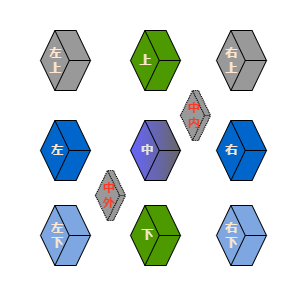
\includegraphics[width=0.85\textwidth]{./images/zi-matrix-CHN.png}
\caption{Figure 1: Zi-Matrix model}
\end{figure}

The decomposition of each character into the Zi-Matrix is performed
manually using a hierarchical approach. This process involves a series
of decomposition steps. First, the character is broken down into its
major components, assigning each to its appropriate position within the
matrix. If a component itself is complex, it is further decomposed,
recursively, into its constituent parts, again assigning them to
positions within a sub-matrix representing that component. This
hierarchical decomposition continues until the most fundamental
components -- those that cannot be reasonably further divided -- are
identified. These fundamental components become candidates for the
``elemental character'' set. This manual, hierarchical approach ensures
a consistent and considered analysis of character structure, leveraging
expert linguistic knowledge to guide the decomposition.

\begin{figure}
\centering
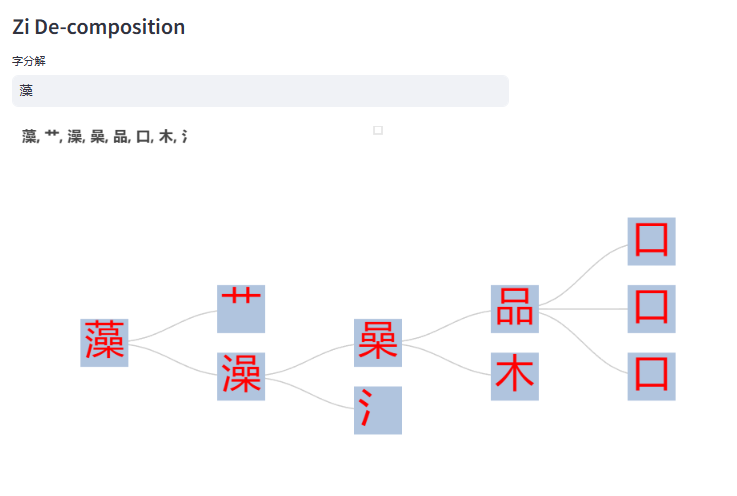
\includegraphics[width=0.85\textwidth]{./images/app_decomposing-zi.png}
\caption{Figure 2: Decompositing an example Chinese character}
\end{figure}

\subsection{Elemental Characters
Analysis}\label{elemental-characters-analysis}

Through manual decomposition of 6190 Chinese characters using the
Zi-Matrix method, we identified 422 unique, irreducible components as
``elemental characters'' (元字). These components represent the
fundamental building blocks that emerged during our hierarchical
decomposition process. Table 1 presents these elemental characters
organized by stroke count, with a clear distinction between traditional
Kangxi radicals and newly identified components.

\subsubsection{Elemental Characters (元字) by Stroke Count and Origin -
Table
1}\label{elemental-characters-ux5143ux5b57-by-stroke-count-and-origin---table-1}

\begin{longtable}[]{@{}
  >{\raggedright\arraybackslash}p{(\columnwidth - 4\tabcolsep) * \real{0.3333}}
  >{\raggedright\arraybackslash}p{(\columnwidth - 4\tabcolsep) * \real{0.3333}}
  >{\raggedright\arraybackslash}p{(\columnwidth - 4\tabcolsep) * \real{0.3333}}@{}}
\toprule\noalign{}
\begin{minipage}[b]{\linewidth}\raggedright
笔画数 (Stroke Count)
\end{minipage} & \begin{minipage}[b]{\linewidth}\raggedright
元字 (Kangxi Radicals)
\end{minipage} & \begin{minipage}[b]{\linewidth}\raggedright
元字 (New Radicals)
\end{minipage} \\
\midrule\noalign{}
\endhead
\bottomrule\noalign{}
\endlastfoot
1 & 丨丶丿乀乁乚乛亅一乙 & \\
2 & 丷亠亻冂冖冫凵⺈刂勹匚匸卩㔾厶讠二人儿入八几刀力匕十卜厂又 &
⺀乂龴⺁丁七乃九了刁 \\
3 &
夂夊宀尢屮巛廴彐彑彡彳忄扌氵丬纟艹辶阝饣口囗土士夕大女子寸小尸山川工己巾干幺广廾弋弓犭门飞马
& 亍兀⺌⺍⻏万丈三上下与个丸义久么之乞也习于亏亡刃勺千叉及已乡才 \\
4 &
攴攵殳灬爫爻爿牜⺩礻禸罓耂心戈戶户手支文斗斤方无日曰月木欠止歹毋比毛氏气水火爪父片牙牛犬王瓦见贝车长韦风
&
旡朩⺧不丑专中丰为乌云五井亢今介仓以元公六内冈凶分办勾勿匀匹区升午友天太夫少尤尺屯巨巴开 \\
5 & 氺疋疒癶罒衤钅母玄玉瓜甘生用田白皮皿目矛矢石示禾穴立鸟龙 &
乍刍戋𤴔且丘丙业东乎乐令兄兰冬出击包北半占卡去古句另只可台四央失头宁它尼市布平必斥旦未末本术正由甲申电 \\
6 & ⺮⺶聿艮虍覀竹米糸缶网羊羽老而耒耳肉臣自至臼舌舟色虫血行衣西页齐 &
囟尧屰⺷交共各合吉向吕寺并庄式曲 \\
7 & 豕豸酉卤舛角言谷豆赤走足身辛辰邑釆里麦龟 &
㐬佥呙坙夆奂孚肙员㕻甫良 \\
8 & 隹黾金阜隶雨青非鱼齿 & 龺幷其奉尚易東责 \\
9 & 面革韭音食首香骨鬼 & 畐咸柬畏禺 \\
10 & 高鬥 & \\
11 & 麻鹿 & \\
12 & 黍黄黑 & \\
13 & 鼓 & \\
14 & 鼻 & \\
\end{longtable}

The identified elemental character set comprises 245 components derived
from the traditional Kangxi radicals system and introduces 177
additional components. This expansion reflects our more granular
approach to character decomposition, where some traditionally grouped
radicals are treated as individual elements. These newly identified
components, though not traditionally recognized as independent units in
standard dictionaries, serve crucial phonetic and/or semantic roles in
character formation. For instance, components like 禺 and 乍, while not
classified as radicals in traditional systems, demonstrate consistent
semantic contributions in compound characters, as we will explore in our
case studies (Section {[}Section Number{]}).

Our elemental character set reveals a finer granularity in Chinese
character composition than the traditional Kangxi system. It encompasses
three main types of components: familiar semantic radicals (e.g.,
氵{[}water{]}, 木{[}wood{]}, 日{[}sun{]}, 月{[}moon{]}, 心{[}heart{]},
手{[}hand{]}, 口{[}mouth{]}), basic structural elements (e.g., 一, 丨,
丿, 丶, 乙, 口, 凵, 冂), and frequently occurring components that carry
both phonetic and semantic information (e.g., 方, 占, 且, 戋, 乍, 禺,
尧, 佥). Some components inherited from the Kangxi system, such as
鼓(drum), while historically significant, may be reconsidered for
practical modern applications. This comprehensive set of elemental
characters provides a more nuanced foundation for understanding and
teaching Chinese character composition, potentially simplifying the
learning process while maintaining semantic integrity.

\subsubsection{Elemental Characters: Occurrence Frequency and
Categorization}\label{elemental-characters-occurrence-frequency-and-categorization}

Analysis of high-frequency elemental characters (with occurrences ≥ 23,
a threshold chosen to include 气 {[}qi/breath/energy{]}, given its
fundamental importance in Chinese philosophy and culture) reveals clear
patterns in character composition. The frequency distribution shows
strong clustering around fundamental human concepts and natural
elements. For instance, in human-related categories (人-), elements like
口 (mouth, 300 occurrences) and 手 (hand, 261 occurrences) show
remarkably high usage rates, reflecting their importance in expressing
human actions and experiences. Similarly, in the natural world
categories, 水 (water, 377 occurrences) and 木 (wood, 324 occurrences)
demonstrate high frequencies, indicating their crucial role in character
formation related to natural phenomena. Notably, 亻(human radical, 213
occurrences) and 女 (female, 137 occurrences) also show high
frequencies, underlining the human-centric nature of character
formation.

\begin{figure}
\centering
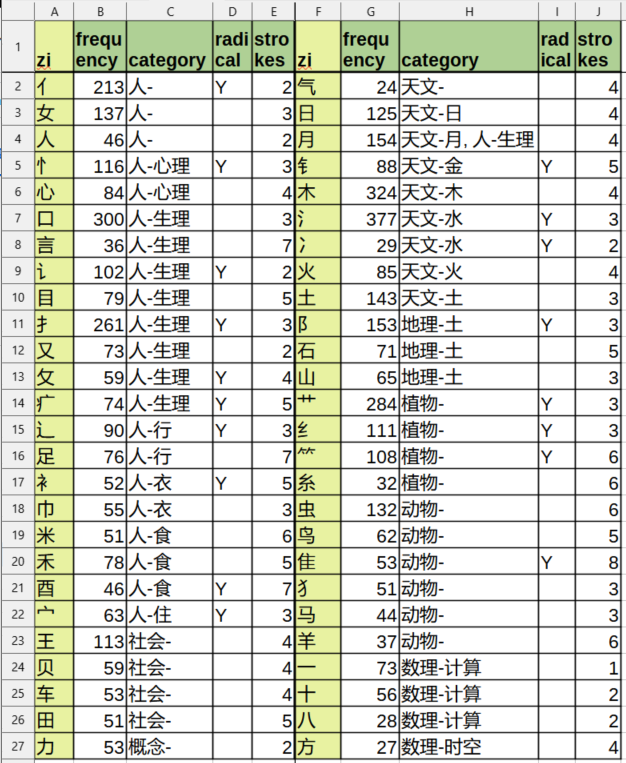
\includegraphics[width=0.85\textwidth]{./images/top-elemental-zi-ENU.png}
\caption{Figure 3: Top elemental characters}
\end{figure}

The categorization system reveals a hierarchical organization centered
on major conceptual domains. The system distinguishes between
human-centered categories (人-系列) including physiological (生理),
psychological (心理), and behavioral (行) aspects; natural elements
(天文-) including the traditional five elements (金木水火土); and
categories for flora (植物-), fauna (动物-), mathematical concepts
(数理-), and abstract concepts (概念-). This classification not only
reflects traditional Chinese philosophical understanding of the world
but also provides a systematic framework for understanding character
composition. Notably, the frequency distribution within these categories
suggests that characters related to human experience and basic natural
elements form the core building blocks of the writing system, while more
specialized or abstract concepts show lower frequencies. The inclusion
of 气 (24 occurrences) in this analysis proves particularly significant,
as it represents a threshold case that bridges fundamental philosophical
concepts with practical character formation patterns.

\subsubsection{Visualizing
Categorization}\label{visualizing-categorization}

\begin{figure}
\centering
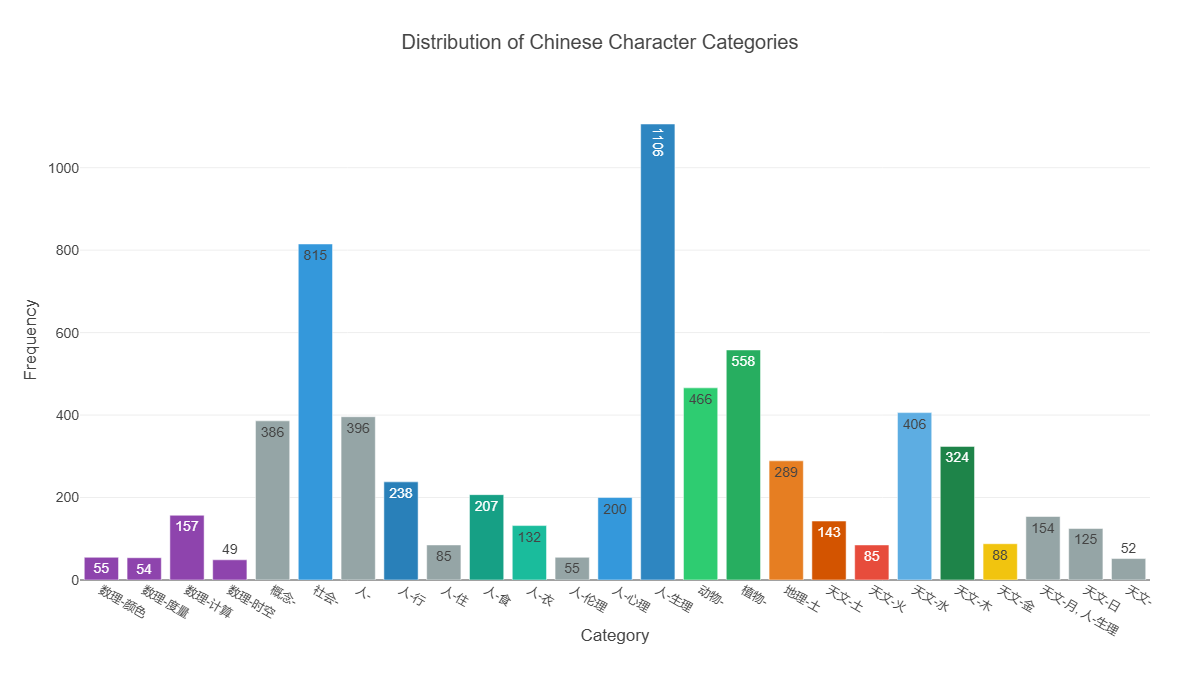
\includegraphics[width=0.85\textwidth]{./images/zi_category_histogram.png}
\caption{Figure 4: Distribution of Chinese characters across conceptual
categories, showing frequency of occurrence ordered from cosmic to human
to abstract realms.}
\end{figure}



The visualization reveals a remarkable pattern in the distribution of
Chinese characters that reflects ancient Chinese cosmological
understanding. Beginning with celestial elements (天文-), the categories
flow through natural phenomena to human experience, creating a narrative
that resonates deeply with traditional Chinese philosophical principles.
The striking prominence of human-related physiological characters
(人-生理, 1106 occurrences) at the center of this distribution, bridged
between natural elements and social constructs, echoes the classical
Chinese view of humans as the connecting point between Heaven and Earth
(天人合一). This central position is flanked by substantial
representations in both natural domains---flora (植物-, 558 occurrences)
and fauna (动物-, 466 occurrences)---and social spheres (社会-, 815
occurrences).

Within the astronomical/natural elements category (天文-), water (水,
406 occurrences) and wood (木, 324 occurrences) show notably higher
frequencies than fire (火), metal (金), and earth (土), suggesting their
greater significance in character formation. The systematic progression
from celestial phenomena through natural elements, human experience, and
finally to abstract mathematical concepts (数理-) reveals an elegant
hierarchical structure that mirrors traditional Chinese cosmological
ordering. This distribution pattern suggests an underlying
organizational principle in Chinese character evolution that reflects
both human cognitive development and natural world observations, a
relationship that will be further explored through its connection to the
Fibonacci sequence.

\subsubsection{Character Compositional
Patterns}\label{character-compositional-patterns}

\begin{figure}
\centering
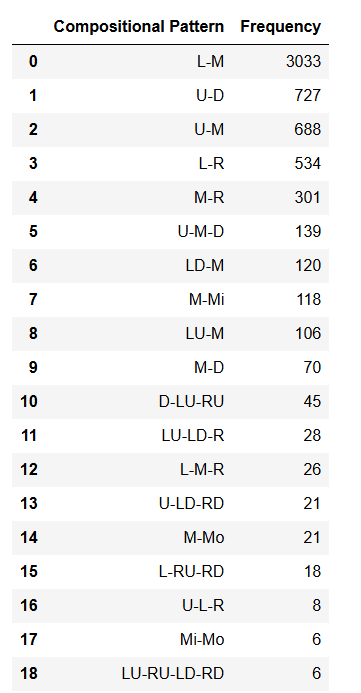
\includegraphics[width=0.85\textwidth]{./images/app_compositional_pattern.png}
\caption{Figure 5: Distribution of Chinese character compositional
patterns, showing frequency of each pattern type.}
\end{figure}



Analysis of character compositions reveals patterns remarkably similar
to molecular organization in nature. Just as atoms combine through
fundamental interactions, elemental characters (元字) interact spatially
to form more complex characters. The most prevalent arrangements mirror
basic two-body interactions, appearing as phonetic-semantic compounds in
various orientations: left-middle (L-M, 3,033 characters), up-down (U-D,
727 characters), up-middle (U-M, 688 characters), and left-right (L-R,
534 characters). These relative positions, while described in modern
directional terms, reflect more fundamental spatial relationships that
transcend the historical evolution from vertical to horizontal writing
systems.

More complex patterns demonstrate sophisticated geometric arrangements
analogous to multi-body interactions in physics. Three-component
interactions manifest in triangular configurations like
down-left\_up-right\_up (D-LU-RU, 45 characters) and
left\_up-left\_down-right (LU-LD-R, 28 characters), while four-component
interactions appear in symmetrical enclosure patterns, though less
frequently (6 characters). This three-dimensional spatial organization
distinguishes Chinese characters from the linear sequence of alphabetic
writing systems, reflecting instead the multi-dimensional interactions
observed in natural systems. The clear preference for simpler two-body
arrangements, followed by decreasing frequency of more complex geometric
patterns, mirrors nature's tendency toward efficient, stable
configurations. This distribution provides valuable insights for both
understanding character formation principles and developing effective
learning strategies based on fundamental spatial relationships.

\subsection{Storytelling Characters}\label{storytelling-characters}

Chinese characters are not merely symbols for recording language; they
are sophisticated vehicles for storytelling that encode observations,
wisdom, and natural principles within their structure. Building upon our
analysis of elemental characters and their compositional patterns, we
now explore how these basic units combine to tell stories at multiple
scales - from individual character families to complete poems. Just as
molecules tell the story of matter's organization through their bonds
and interactions, Chinese characters reveal deeper narratives through
their semantic relationships and evolving combinations. This section
examines how meaning emerges through increasingly complex arrangements:
from character families that share common elements, through network-like
compound formations, to the crystalline structures of classical poetry.
Each level demonstrates how Chinese writing, like natural systems,
achieves remarkable efficiency in encoding information while maintaining
profound aesthetic and philosophical coherence.

\subsubsection{3.1 Case Studies - Composite
Characters}\label{case-studies---composite-characters}

\paragraph{3.1.1 The 日 Family}\label{the-ux65e5-family}

\begin{figure}
\centering
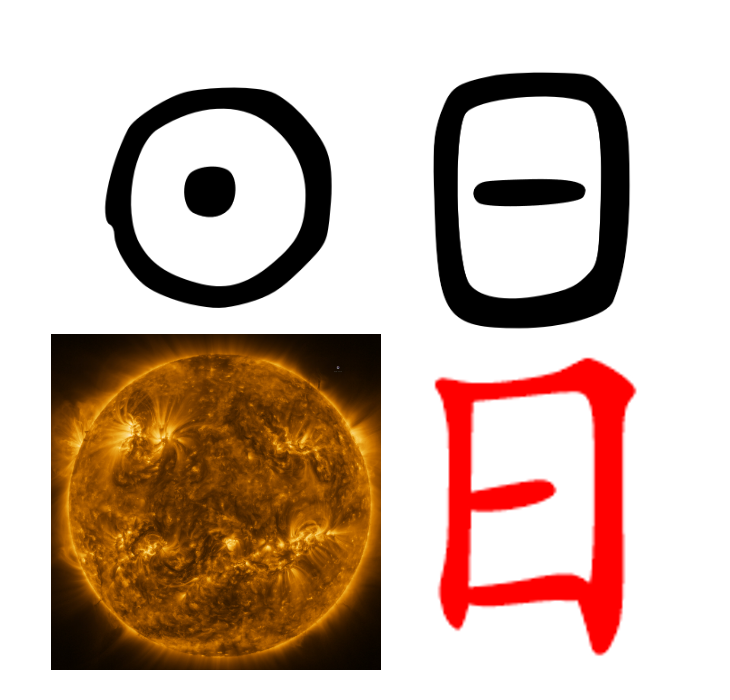
\includegraphics[width=0.5\textwidth]{./images/zi_sun.png}
\caption{Figure 6: Evolution of the character 日 (sun) from oracle bone
pictograph to modern form, alongside actual solar image}
\end{figure}



The Chinese character ``日'' (rì), meaning ``sun'' or ``day'', serves as
a powerful illustration of how Chinese characters efficiently encode
natural observations and knowledge. The character's evolution from its
oracle bone pictograph---depicting a circular sun with a central
dot---to its modern form demonstrates remarkable preservation of core
visual concepts while gaining calligraphic efficiency.

\begin{longtable}[]{@{}
  >{\raggedright\arraybackslash}p{(\columnwidth - 6\tabcolsep) * \real{0.2093}}
  >{\raggedright\arraybackslash}p{(\columnwidth - 6\tabcolsep) * \real{0.2093}}
  >{\raggedright\arraybackslash}p{(\columnwidth - 6\tabcolsep) * \real{0.3721}}
  >{\raggedright\arraybackslash}p{(\columnwidth - 6\tabcolsep) * \real{0.2093}}@{}}
\toprule\noalign{}
\begin{minipage}[b]{\linewidth}\raggedright
Formula
\end{minipage} & \begin{minipage}[b]{\linewidth}\raggedright
Meaning
\end{minipage} & \begin{minipage}[b]{\linewidth}\raggedright
Natural Insight
\end{minipage} & \begin{minipage}[b]{\linewidth}\raggedright
Pinyin
\end{minipage} \\
\midrule\noalign{}
\endhead
\bottomrule\noalign{}
\endlastfoot
日 + 月 = 明 & bright & Sun and moon as primary celestial light sources
& míng \\
日 + 正 = 是 & to be/truth & Overhead sun casts no shadows, revealing
true form & shì \\
知 + 日 = 智 & wisdom & The sun radiates energy without depletion,
demonstrating how true wisdom transcends accumulated knowledge to
understand principles of sustainable benefit & zhì \\
日 + 日 + 日 = 晶 & crystal/bright & Intensification of light/clarity
through repetition & jīng \\
门 + 日 = 间 & space/interval & Light revealing space between door
frames & jiān \\
日 + 寸 = 时 & time & Sun's shadow measure in ancient timekeeping &
shí \\
日 + 生 = 星 & star & Stars as celestial light producers & xīng \\
丿 + 日 = 白 & white & Pure light emanating from sun & bái \\
日 + 一 = 旦 & dawn & Sun rising above horizon & dàn \\
九 + 日 = 旭 & rising sun & Multiple rays of morning sunlight & xù \\
日 + 十 = 早 & early & Sun above treetops at dawn & zǎo \\
日 + 干 = 旱 & drought & Intense sun causing dryness & hàn \\
三 + 八 + 日 = 春 & spring & Sunlight causing seeds to break soil &
chūn \\
\end{longtable}

\begin{figure}
\centering
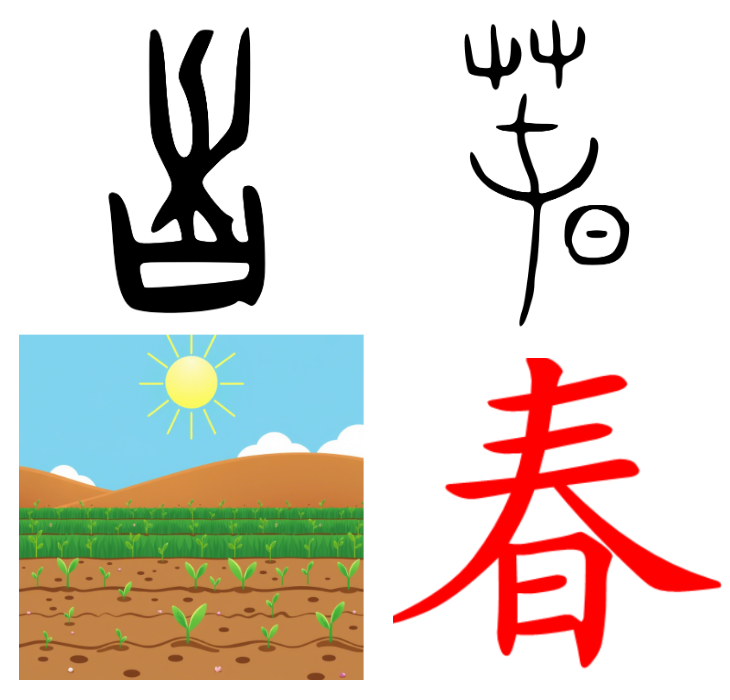
\includegraphics[width=0.5\textwidth]{./images/zi_spring.png}
\caption{Figure 7: The character 春 (spring) captures multiple aspects of
seasonal transition}
\end{figure}



The character 春 (spring) exemplifies efficient semantic encoding
through its components: 三 (representing multiple aspects - abundance of
sprouting life, layers of frozen earth), 八 (break/split), and 日 (sun).
Together, these elements capture the dynamics of spring's arrival - the
interaction between strengthening sunlight, earth's layers, and emerging
life. This structure demonstrates how Chinese characters can layer
multiple related meanings within a single, coherent form.

\paragraph{3.1.2 The 坙 Family}\label{the-ux5759-family}

\begin{figure}
\centering
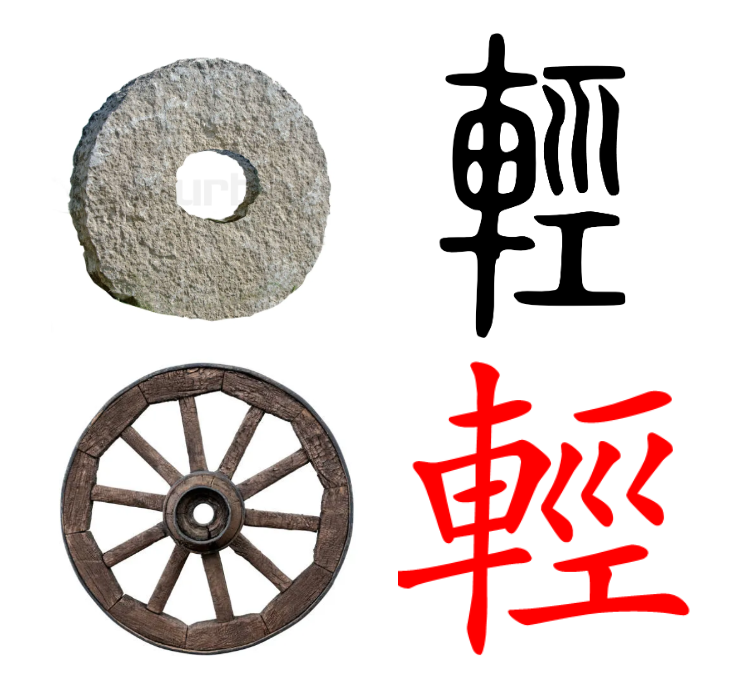
\includegraphics[width=0.5\textwidth]{./images/zi_stem.png} 
\caption{Figure 8: The character 坙
encodes the evolution from material mass to structural efficiency}
\end{figure}

The character 坙 exemplifies how Chinese writing preserves fundamental
principles of human innovation. Beyond its basic meaning of ``core'' and
``lightness,'' this character documents a critical transition in human
understanding: the discovery that effectiveness comes from optimized
structure rather than raw mass. The progression from solid stone wheels
to spoked wooden designs represents both technological advancement and
conceptual breakthrough - the recognition that core principles often
emerge through reduction rather than addition.

\begin{longtable}[]{@{}
  >{\raggedright\arraybackslash}p{(\columnwidth - 6\tabcolsep) * \real{0.1731}}
  >{\raggedright\arraybackslash}p{(\columnwidth - 6\tabcolsep) * \real{0.1731}}
  >{\raggedright\arraybackslash}p{(\columnwidth - 6\tabcolsep) * \real{0.4808}}
  >{\raggedright\arraybackslash}p{(\columnwidth - 6\tabcolsep) * \real{0.1731}}@{}}
\toprule\noalign{}
\begin{minipage}[b]{\linewidth}\raggedright
Formula
\end{minipage} & \begin{minipage}[b]{\linewidth}\raggedright
Meaning
\end{minipage} & \begin{minipage}[b]{\linewidth}\raggedright
Natural/Technical Insight
\end{minipage} & \begin{minipage}[b]{\linewidth}\raggedright
Pinyin
\end{minipage} \\
\midrule\noalign{}
\endhead
\bottomrule\noalign{}
\endlastfoot
气 + 坙 = 氢 & hydrogen & Simplest element with single proton core &
qīng \\
艹 + 坙 = 茎 & plant stem & Essential structural support maintaining
plant integrity & jīng \\
纟 + 坙 = 经 & classic texts/meridian & Core texts that weave through
cultural/anatomical fabric & jīng \\
坙 + 力 = 劲 & strength/vigor & How core fibers generate physical power
& jìn \\
坙 + 页 = 颈 & neck & Crucial connecting structure between body and
brain & jǐng \\
彳 + 坙 = 径 & path/radius & Most direct route from center to periphery
& jìng \\
车 + 坙 = 轻 & light(weight) & Structural efficiency through essential
components & qīng \\
\end{longtable}

This character family demonstrates the Chinese writing system's capacity
to encode and transmit complex principles across generations. Each
derivative character extends the core concept of structural efficiency
into different domains, from atomic physics (氢) to biological systems
(茎), preserving not just the end results but the underlying principles
of innovation.

\paragraph{3.1.3 The 禺 Family}\label{the-ux79ba-family}

\begin{figure}
\centering
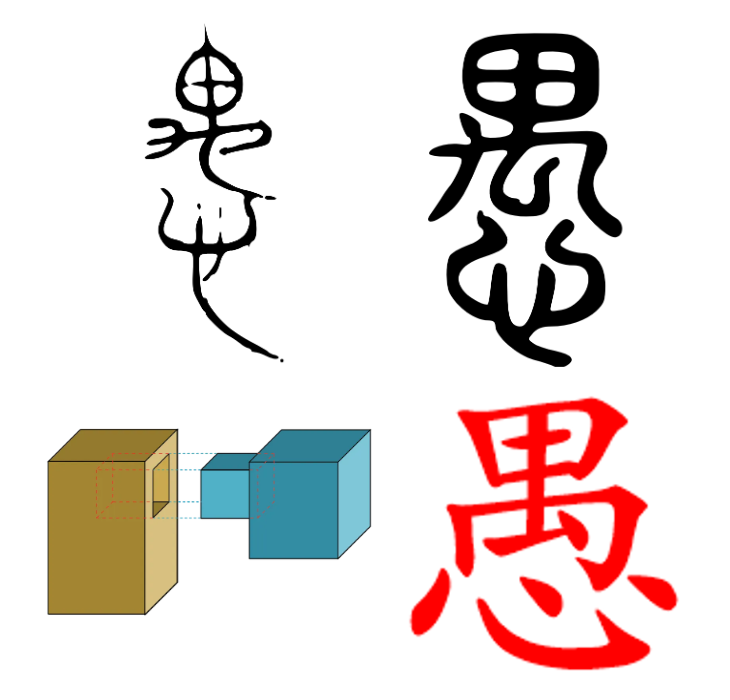
\includegraphics[width=0.5\textwidth]{./images/zi_join.png} 
\caption{Figure 9: The character 禺
evolution, depicting fundamental concept of joining/coupling}
\end{figure}

The character 禺 represents a fundamental concept of joining or coupling
in Chinese writing, functioning as a semantic force carrier for various
types of connections and interactions.

\begin{longtable}[]{@{}
  >{\raggedright\arraybackslash}p{(\columnwidth - 6\tabcolsep) * \real{0.1731}}
  >{\raggedright\arraybackslash}p{(\columnwidth - 6\tabcolsep) * \real{0.1731}}
  >{\raggedright\arraybackslash}p{(\columnwidth - 6\tabcolsep) * \real{0.4808}}
  >{\raggedright\arraybackslash}p{(\columnwidth - 6\tabcolsep) * \real{0.1731}}@{}}
\toprule\noalign{}
\begin{minipage}[b]{\linewidth}\raggedright
Formula
\end{minipage} & \begin{minipage}[b]{\linewidth}\raggedright
Meaning
\end{minipage} & \begin{minipage}[b]{\linewidth}\raggedright
Natural/Physical Insight
\end{minipage} & \begin{minipage}[b]{\linewidth}\raggedright
Pinyin
\end{minipage} \\
\midrule\noalign{}
\endhead
\bottomrule\noalign{}
\endlastfoot
亻 + 禺 = 偶 & 1. couple/partner; 2. chance/accident; 3. even number &
Captures both intentional pairing and chance encounters, while `even
numbers' suggests balanced states & ǒu \\
宀 + 禺 = 寓 & dwelling/metaphor & Physical space enabling connections &
yù \\
辶 + 禺 = 遇 & encounter/meet & Dynamic interaction through movement &
yù \\
禺 + 心 = 愚 & inability to connect & Cognitive dimension of connection
& yú \\
阝 + 禺 = 隅 & corner/intersection & Spatial manifestation of joining &
yú \\
耒 + 禺 = 耦 & linked roots & Natural systems demonstrating connection &
ǒu \\
\end{longtable}

This character family demonstrates how Chinese writing conceptualizes
different types of connections - from physical joining to spatial
relationships to cognitive associations - all derived from a single
fundamental concept of coupling.

\paragraph{3.1.4 The 乍 Family}\label{the-ux4e4d-family}

\begin{figure}
\centering
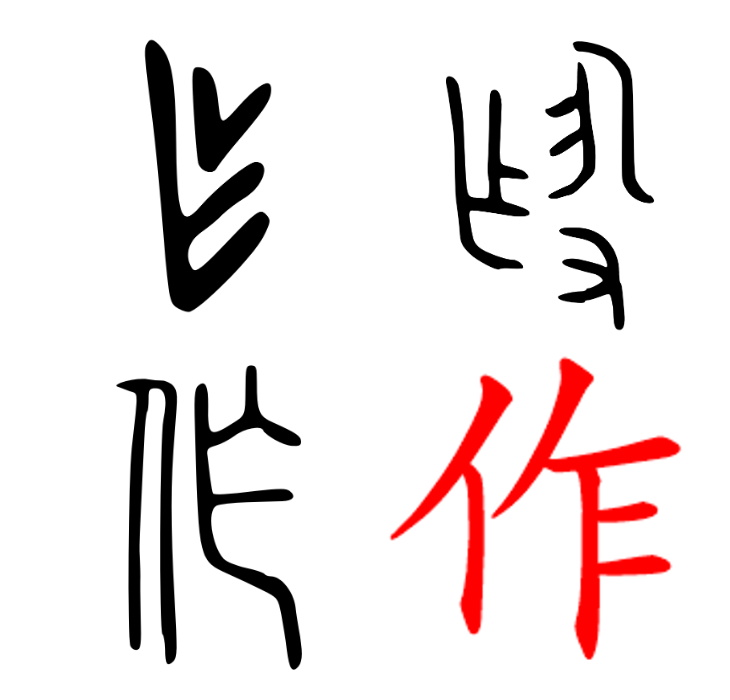
\includegraphics[width=0.5\textwidth]{./images/zi_work.png}
\caption{Figure 10: Evolution of
character 乍 (work/make) from oracle bone to modern form}
\end{figure}

The character 乍 represents fundamental concepts of work, creation, and
transformation. Its historical forms suggest the process of making or
transforming materials, functioning as a semantic force carrier for
various types of productive activity.

\begin{longtable}[]{@{}
  >{\raggedright\arraybackslash}p{(\columnwidth - 6\tabcolsep) * \real{0.1731}}
  >{\raggedright\arraybackslash}p{(\columnwidth - 6\tabcolsep) * \real{0.1731}}
  >{\raggedright\arraybackslash}p{(\columnwidth - 6\tabcolsep) * \real{0.4808}}
  >{\raggedright\arraybackslash}p{(\columnwidth - 6\tabcolsep) * \real{0.1731}}@{}}
\toprule\noalign{}
\begin{minipage}[b]{\linewidth}\raggedright
Formula
\end{minipage} & \begin{minipage}[b]{\linewidth}\raggedright
Meaning
\end{minipage} & \begin{minipage}[b]{\linewidth}\raggedright
Natural/Physical Insight
\end{minipage} & \begin{minipage}[b]{\linewidth}\raggedright
Pinyin
\end{minipage} \\
\midrule\noalign{}
\endhead
\bottomrule\noalign{}
\endlastfoot
亻 + 乍 = 作 & to make/to do & Direct human productive activity & zuò \\
日 + 乍 = 昨 & yesterday & Time transformed through work completed &
zuó \\
乍 + 心 = 怎 & how? & Mental process of problem-solving & zěn \\
火 + 乍 = 炸 & to explode/to fry & Energy transformation in different
scales & zhà \\
讠 + 乍 = 诈 & to deceive & Misuse of effort in communication & zhà \\
口 + 乍 = 咋 & how (colloquial) & Verbal expression of questioning
process & zǎ \\
酉 + 乍 = 酢 & vinegar & Chemical transformation through work & zuò \\
⺮ + 乍 = 笮 & to press & Physical work applied to materials & zé \\
穴 + 乍 = 窄 & narrow & Spatial transformation through constraint &
zhǎi \\
\end{longtable}

This family demonstrates how a basic concept of work/transformation
generates characters spanning physical, chemical, mental, temporal, and
social domains - much like how energy manifests in different forms
throughout nature.

\paragraph{3.1.5 The 寺 Family}\label{the-ux5bfa-family}

\begin{figure}
\centering
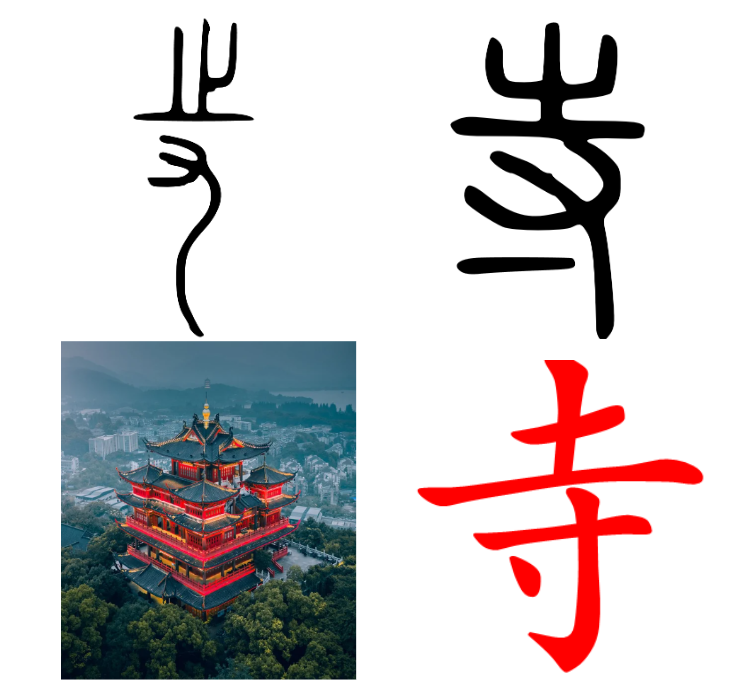
\includegraphics[width=0.5\textwidth]{./images/zi_temple.png}
\caption{Figure 11: Evolution of character 寺 (temple) from oracle bone
script to modern form, with example of traditional temple architecture}
\end{figure}



The character 寺, originally depicting a temple or place of authority,
functions as a semantic carrier representing ordered structure and
measured interaction. Its architectural origins in temple design suggest
principles of balance, hierarchy, and measured sacred space.

\begin{longtable}[]{@{}
  >{\raggedright\arraybackslash}p{(\columnwidth - 6\tabcolsep) * \real{0.1636}}
  >{\raggedright\arraybackslash}p{(\columnwidth - 6\tabcolsep) * \real{0.1636}}
  >{\raggedright\arraybackslash}p{(\columnwidth - 6\tabcolsep) * \real{0.5091}}
  >{\raggedright\arraybackslash}p{(\columnwidth - 6\tabcolsep) * \real{0.1636}}@{}}
\toprule\noalign{}
\begin{minipage}[b]{\linewidth}\raggedright
Formula
\end{minipage} & \begin{minipage}[b]{\linewidth}\raggedright
Meaning
\end{minipage} & \begin{minipage}[b]{\linewidth}\raggedright
Natural/Architectural Insight
\end{minipage} & \begin{minipage}[b]{\linewidth}\raggedright
Pinyin
\end{minipage} \\
\midrule\noalign{}
\endhead
\bottomrule\noalign{}
\endlastfoot
日 + 寺 = 時 & time as cosmic law & Temple's ritualistic measurement of
sun's movement reveals time as an inescapable cosmic order that governs
all existence - a fundamental principle that commands universal respect
and submission & shí \\
牜 + 寺 = 特 & special/extraordinary & Cattle as precious agricultural
asset offered to temple represents highest form of ritual sacrifice and
distinction & tè \\
亻 + 寺 = 侍 & to serve with ritual propriety & Models service
relationships on temple's hierarchical spatial organization of
inner/outer courts & shì \\
扌 + 寺 = 持 & to uphold/maintain with stability & Reflects temple
architecture's balanced distribution of structural forces and sustained
equilibrium & chí \\
彳 + 寺 = 待 & to await at proper position & Like prescribed positions
in temple processions, represents disciplined positioning in space-time
& dài \\
⺮ + 寺 = 等 & ordered ranking/classification & Mirrors temple
architecture's clear demarcation of sacred spaces by rank and function &
děng \\
山 + 寺 = 峙 & to tower with dignity & Embodies temple pagoda's vertical
presence as symbol of spiritual and moral elevation & zhì \\
忄 + 寺 = 恃 & to depend upon with confidence & Like temple foundations,
represents reliable structural support extended to mental realm & shì \\
讠 + 寺 = 诗 & poetry as sacred architecture & Words arranged with
temple-like precision to create spaces of transcendent meaning & shī \\
\end{longtable}

The 寺 family reveals how temple architecture's principles of structure
and order extend into cosmic time (時), ritual significance (特), social
hierarchies (侍), and artistic expression (诗). This progression from
physical to abstract domains demonstrates the sophisticated metaphorical
thinking in Chinese character formation.

\subsubsection{3.2 Case Studies - Pinyin - A
Counter-Argument}\label{case-studies---pinyin---a-counter-argument}

In the Chinese language, sound (声 shēng), form (形 xíng), and meaning
(意 yì) are all integral components of a vibrant, living system.
Over-emphasizing any single aspect at the expense of the others would be
inefficient, misguided, and unwise. While the Pinyin romanization system
has undeniably augmented the Chinese language by integrating Latin
phonetic components, relying solely on Pinyin and abandoning Chinese
characters would result in a tremendous loss of semantic meaning and
cultural wisdom. The limitations of a purely phonetic system become
apparent below using cases of homophony:

\begin{enumerate}
\def\labelenumi{\arabic{enumi}.}
\tightlist
\item
  Single-character homophony:

  \begin{itemize}
  \tightlist
  \item
    mā: 妈 (mother), 蚂 (ant), 马 (mǎ, horse), 骂 (mà, yell or curse)
  \item
    shì: 是 (to be), 事 (matter), 市 (market), 式 (style), 世 (world)
  \item
    yì: 意 (meaning), 义 (righteousness), 艺 (art), 易 (change)
  \end{itemize}
\item
  Compound-word disambiguation:

  \begin{itemize}
  \tightlist
  \item
    ``xiansheng'' in Pinyin could represent:

    \begin{itemize}
    \tightlist
    \item
      先生 (teacher/mister)
    \item
      现生 (present life)
    \item
      献身 (sacrifice oneself)
    \end{itemize}
  \end{itemize}
\end{enumerate}

Chinese characters, in their elegance and complexity, encode both visual
and auditory information while preserving crucial semantic distinctions.
This harmonious integration of form and function has sustained the
language for millennia. The path forward lies in preserving this
sophisticated writing system while thoughtfully incorporating modern
tools like Pinyin as complementary aids rather than replacements.

\subsubsection{3.3 Case Studies - Characters and
Phrases}\label{case-studies---characters-and-phrases}

Just as matter organizes itself into increasingly complex structures -
from atoms to molecules to molecular clusters - language exhibits
similar emergent properties at different scales. Individual characters
(字) serve as the atomic units, carrying fundamental meanings and
combining properties. These form compounds and phrases (词组), analogous
to molecules with stable semantic bonds. At a higher level of
organization, these linguistic molecules arrange themselves into
sophisticated structures like poems, which, like molecular clusters,
exhibit properties beyond the sum of their parts. This natural hierarchy
of meaning-making demonstrates the living, self-organizing nature of
Chinese language.

\paragraph{3.3.1 The 子 Family}\label{the-ux5b50-family}

\begin{figure}
\centering
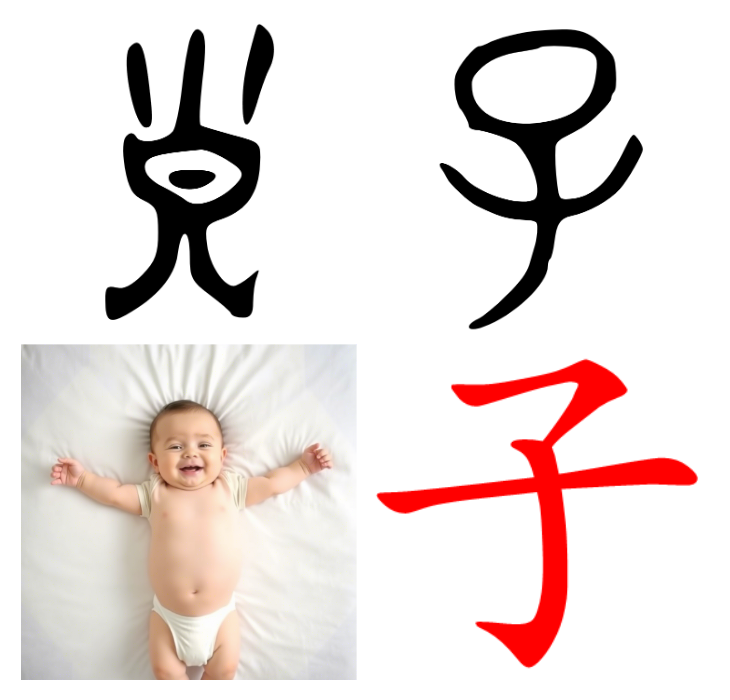
\includegraphics[width=0.5\textwidth]{./images/zi_child.png}

\caption{Figure 12: Evolution of character 子 (child) from oracle bone
script to modern form, with visual metaphor of a baby with outstretched
arms}

\end{figure}


\begin{longtable}[]{@{}
  >{\raggedright\arraybackslash}p{(\columnwidth - 6\tabcolsep) * \real{0.1731}}
  >{\raggedright\arraybackslash}p{(\columnwidth - 6\tabcolsep) * \real{0.1731}}
  >{\raggedright\arraybackslash}p{(\columnwidth - 6\tabcolsep) * \real{0.4808}}
  >{\raggedright\arraybackslash}p{(\columnwidth - 6\tabcolsep) * \real{0.1731}}@{}}
\toprule\noalign{}
\begin{minipage}[b]{\linewidth}\raggedright
Formula
\end{minipage} & \begin{minipage}[b]{\linewidth}\raggedright
Meaning
\end{minipage} & \begin{minipage}[b]{\linewidth}\raggedright
Natural/Cultural Insight
\end{minipage} & \begin{minipage}[b]{\linewidth}\raggedright
Pinyin
\end{minipage} \\
\midrule\noalign{}
\endhead
\bottomrule\noalign{}
\endlastfoot
女 + 子 = 好 & good/well & Child with mother represents fundamental
goodness & hǎo \\
耂 + 子 = 孝 & filial piety & Elder above child shows respect and care &
xiào \\
子 + 小 = 孙 & grandson & Small child represents generational
continuation & sūn \\
木 + 子 = 李 & plum tree & Fruit as nature's offspring & lǐ \\
米 + 子 = 籽 & seed & Grain's offspring, agricultural reproduction &
zǐ \\
禾 + 子 = 季 & season & Crop cycle marked by growth stages & jì \\
宀 + 子 = 字 & character & Child under roof represents nurturing of
knowledge & zì \\
小 + 冖 + 子 = 学 & to learn/study & Child (子) under shelter (冖)
starting small (小) captures the essence of education & xué \\
\end{longtable}

The character 子 (zǐ), originally depicting a child with outstretched
arms, functions as both a semantic and phonetic component in character
formation. Its visual evolution preserves the core meaning of offspring
while extending into broader domains of growth and nurturing.

\paragraph{3.3.2 The 子 Network}\label{the-ux5b50-network}

\begin{figure}
\centering
\includegraphics[width=0.5\textwidth]{./images/zi_child-phrase.png}
\caption{Figure 13: Semantic extensions of 子 across various domains}
\end{figure}



\begin{longtable}[]{@{}
  >{\raggedright\arraybackslash}p{(\columnwidth - 6\tabcolsep) * \real{0.1961}}
  >{\raggedright\arraybackslash}p{(\columnwidth - 6\tabcolsep) * \real{0.2157}}
  >{\raggedright\arraybackslash}p{(\columnwidth - 6\tabcolsep) * \real{0.3725}}
  >{\raggedright\arraybackslash}p{(\columnwidth - 6\tabcolsep) * \real{0.2157}}@{}}
\toprule\noalign{}
\begin{minipage}[b]{\linewidth}\raggedright
Category
\end{minipage} & \begin{minipage}[b]{\linewidth}\raggedright
Compounds
\end{minipage} & \begin{minipage}[b]{\linewidth}\raggedright
Semantic Extension
\end{minipage} & \begin{minipage}[b]{\linewidth}\raggedright
Examples
\end{minipage} \\
\midrule\noalign{}
\endhead
\bottomrule\noalign{}
\endlastfoot
Human Relations & 父子, 子女, 子孙, 弟子 & Core family ties &
father-and-son, children, descendants, disciple \\
Honorific Terms & 老子, 孔子, 墨子, 孙子, 君子 & Respect and wisdom &
Master, great teachers, gentlement \\
Scientific Objects & 量子, 光子, 原子, 电子 & Fundamental particles &
Atom, quantum, electron \\
Mathematical Objects & 因子, 子集, 子空间 & Math concepts & factor,
subset, sub-space \\
Natural Elements & 种子, 脑子, 芽子, 子宫 & Biological growth & Seed,
brain, sprout, womb \\
Animals & 狮子, 兔子, 蚊子 & living objects & Lion, rabbit, mosquito \\
Tools/Objects & 筷子, 梯子, 桌子, 房子, 子弹 & Functional items &
Chopsticks, ladder, table, house, bullet \\
Time Concepts & 日子, 子时, 甲子 & Temporal cycles & Days, midnight
hour, 60-year cycle \\
Aggressor & 日本鬼子, 毛子 & Nicknames & Japanese soldier, northern
invader \\
\end{longtable}

This analysis reveals how 子 extends from its concrete meaning of
``child'' into an extraordinarily rich semantic network spanning
natural, social, and abstract domains. At the foundational level, it
captures core human relationships (父子, 子女) and biological growth
(种子, 子宫). Its semantic scope then expands remarkably to encompass
everything from the cosmic scale of fundamental particles (量子, 原子)
to the precision of mathematical abstractions (因子, 子集). The
character's versatility is further demonstrated in its application to
everyday objects (筷子, 房子), temporal concepts (日子, 甲子), and even
cultural-historical contexts (日本鬼子). What's particularly striking is
how 子 maintains its core associations with growth, fundamentality, and
belonging across these diverse domains - whether describing a physical
descendant (孙子), an intellectual lineage (弟子), or the smallest units
of matter (原子). This semantic radiation from concrete to abstract
meanings, while preserving core conceptual links, exemplifies the
sophisticated metaphorical thinking embedded in Chinese character
evolution and compound formation.

\subsubsection{3.4 Case Studies - Poems: Temple of
Words}\label{case-studies---poems-temple-of-words}

This section examines how classical Chinese poetry achieves remarkable
semantic density through minimal character usage. The survival of these
poems across millennia demonstrates powerful principles of cultural
selection, where maximum meaning with minimum structure creates enduring
linguistic artwork.

\paragraph{3.4.1 Poetry as Sacred
Architecture}\label{poetry-as-sacred-architecture}

\texttt{讠\ +\ 寺\ =\ 诗}: This elegant formation captures the essence
of poetry - the construction of linguistic temples where carefully
chosen words create spaces of meaning that transcend their components.
Just as temples transform physical space into sacred realm through
architectural principles, classical Chinese poems create meaning through
precise structural arrangement.

\begin{figure}
\centering
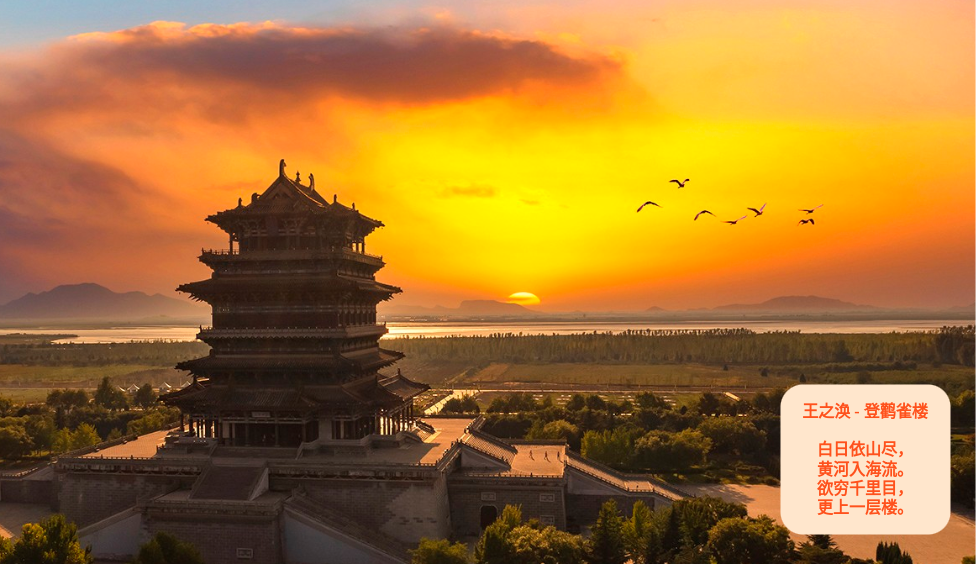
\includegraphics[width=0.85\textwidth]{./images/poem_huang-he-lou.png}
\caption{Figure 14: Magnificant Huang He Lou}
\end{figure}

\begin{verbatim}
(III) 王之涣 - 登鹳雀楼

白日依山尽,
黄河入海流。
欲穷千里目,
更上一层楼。
\end{verbatim}

\begin{figure}
\centering
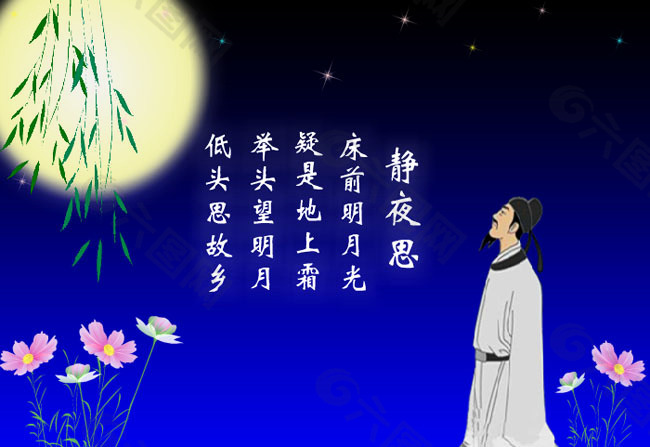
\includegraphics[width=0.85\textwidth]{./images/poem_moonlight.jpg}
\caption{Figure 15: Deep Thought under Moonlight}
\end{figure}

\begin{verbatim}
(IV) 李白 - 静夜思

床前明月光,
疑是地上霜。
举头望明月,
低头思故乡。
\end{verbatim}

When this author queries AI systems for exemplary Chinese poems, these
two masterpieces emerge with remarkable frequency, suggesting their
special status in the corpus of Chinese literature.

\paragraph{3.4.2 Architectural Principles of Poetic
Construction}\label{architectural-principles-of-poetic-construction}

\subparagraph{3.4.2.1 Foundation (地基)}\label{foundation-ux5730ux57fa}

\begin{itemize}
\tightlist
\item
  Elementary Characters as Building Blocks

  \begin{itemize}
  \tightlist
  \item
    Natural elements: 山, 河, 日, 月
  \item
    Basic actions: 上, 望, 举, 低
  \item
    Core concepts: 目, 光, 头, 楼
  \end{itemize}
\end{itemize}

\subparagraph{3.4.2.2 Vertical Progression
(层进)}\label{vertical-progression-ux5c42ux8fdb}

\begin{itemize}
\tightlist
\item
  Physical and Spiritual Elevation

  \begin{itemize}
  \tightlist
  \item
    ``登鹳雀楼'': Literal ascent mirrors expanding consciousness
  \item
    ``静夜思'': Movement from earth (霜) to heaven (月) to heart (思)
  \end{itemize}
\item
  Each level adds new dimension of meaning
\end{itemize}

\subparagraph{3.4.2.3 Sacred Space
(空间)}\label{sacred-space-ux7a7aux95f4}

Both poems create vast mental landscapes through minimal means: -
Horizontal expanse: 千里目, 入海流 - Vertical dimension: 一层楼, 举头望
- Internal realm: 思故乡

\paragraph{3.4.3 Yin-Yang Duality in
Expression}\label{yin-yang-duality-in-expression}

These poems together form a complete cognitive framework through
complementary approaches:

\begin{longtable}[]{@{}
  >{\raggedright\arraybackslash}p{(\columnwidth - 4\tabcolsep) * \real{0.1667}}
  >{\raggedright\arraybackslash}p{(\columnwidth - 4\tabcolsep) * \real{0.4375}}
  >{\raggedright\arraybackslash}p{(\columnwidth - 4\tabcolsep) * \real{0.3958}}@{}}
\toprule\noalign{}
\begin{minipage}[b]{\linewidth}\raggedright
Aspect
\end{minipage} & \begin{minipage}[b]{\linewidth}\raggedright
Yang (阳) - 登鹳雀楼
\end{minipage} & \begin{minipage}[b]{\linewidth}\raggedright
Yin (阴) - 静夜思
\end{minipage} \\
\midrule\noalign{}
\endhead
\bottomrule\noalign{}
\endlastfoot
Celestial Bodies & Sun setting (白日依山) & Moon reflecting (明月光) \\
Movement & Upward progression (更上一层楼) & Circular motion
(举头\ldots 低头) \\
Philosophy & Active pursuit of transcendence & Passive reception of
insight \\
Emotion & Aspiration toward horizons & Nostalgia and connection \\
\end{longtable}

\paragraph{3.4.4 Evolutionary Fitness
Factors}\label{evolutionary-fitness-factors}

The remarkable survival and transmission of these poems can be
attributed to several adaptive advantages:

\subparagraph{3.4.4.1 Structural
Efficiency}\label{structural-efficiency}

\begin{itemize}
\tightlist
\item
  Semantic Density: Maximum meaning in minimum space (20 characters)
\item
  Progressive Construction: From observation to insight
\item
  Information Compression: Multiple layers of meaning per character
\item
  Mnemonic Design: Rhythm and imagery supporting memory
\end{itemize}

\subparagraph{3.4.4.2 Cultural Transmission
Vectors}\label{cultural-transmission-vectors}

\begin{itemize}
\tightlist
\item
  Educational Value

  \begin{itemize}
  \tightlist
  \item
    Accessible characters (易懂) with sophisticated craft (难工)
  \item
    Clear structure supporting memorization (朗朗上口)
  \item
    Universal themes ensuring relevance (代代相传)
  \end{itemize}
\item
  Cognitive Resonance

  \begin{itemize}
  \tightlist
  \item
    Alignment with fundamental thought patterns
  \item
    Balance of concrete and abstract elements
  \item
    Integration of emotion and insight
  \end{itemize}
\end{itemize}

\subparagraph{3.4.4.3 Complementary Wisdom
Paths}\label{complementary-wisdom-paths}

These masterpieces encode two essential approaches to understanding:

\begin{itemize}
\tightlist
\item
  ``登鹳雀楼'': Transcendence Through Effort

  \begin{itemize}
  \tightlist
  \item
    Physical elevation as metaphor for understanding
  \item
    Active engagement with limitations
  \item
    Expansion of perspective through deliberate action
  \end{itemize}
\item
  ``静夜思'': Insight Through Reflection

  \begin{itemize}
  \tightlist
  \item
    Quiet observation revealing deep connection
  \item
    Natural phenomena evoking emotional truth
  \item
    Stillness as path to profound understanding
  \end{itemize}
\end{itemize}

\paragraph{3.4.5 Summary}\label{summary}

These poems demonstrate the sophisticated architecture of classical
Chinese poetry, where careful arrangement of minimal elements creates
enduring structures of meaning. Their survival through millennia
reflects both their remarkable efficiency in encoding wisdom and their
resonance with fundamental patterns of human experience and
understanding. Like well-designed temples, they transform simple
elements into spaces of deep meaning, achieving maximum impact on
culture and civilization.

\subsection{Natural Evolution of
Characters}\label{natural-evolution-of-characters}

In our earlier sections on ``Visualizing Categorization'' and
``Character Compositional Patterns'', we observed how elemental
characters reflect human cognition about nature, how elemental
characters interact like simple objects in the physical world. Here we
explore how Chinese characters may have evolved naturally.

\subsubsection{Historical Context}\label{historical-context}

According to legend, Cangjie invented Chinese characters. Cangjie was a
historian to the Yellow Emperor of China in the 27th century BCE. -
Cangjie was inspired by the natural world, including animal tracks,
landscapes, and the stars. - He believed that if he could capture the
unique features of everything in a single painting, he could create a
writing system. - Cangjie was frustrated with the limitations of
knotting, which was the previous method of recording information. As a
milestone event, Cangjie undoubtedly contributed to the creation of
Chinese writing system. In the grand scheme of a human language, Chinese
characters may have evolved naturally, generation after generation.

\subsubsection{Natural Growth Patterns in Character
Evolution}\label{natural-growth-patterns-in-character-evolution}

Just as natural systems evolve from simple to complex through
predictable patterns, Chinese characters demonstrate similar organic
development. The Fibonacci sequence (1,1,2,3,5,8,13,21,34,\ldots)
provides an elegant framework for understanding this evolution, not as a
rigid mathematical correspondence, but as a metaphor for how complexity
emerges from simplicity in systematic ways.

The accompanying images of Fibonacci patterns in nature - from sunflower
seed arrangements to nautilus shells, from fern fronds to spiral
galaxies - reveal this universal principle of growth and organization.
This same principle can illuminate our understanding of how Chinese
characters evolved from Cangjie's initial inspiration to their current
form.

\begin{figure}
\centering
\includegraphics[width=0.85\textwidth]{./images/fibonacci-spiral-2.png}
\caption{Figure 16: Fibonacci Spiral Patterns in Nature}
\end{figure}

Inspired by universal natural growth pattern like Fibonacci sequence,
this author borrows the sequence to organize Chinese characters in a
similar natural progression: from simple pictographs to sophisticated
composite characters, from concrete objects to abstract concepts. This
natural progression is not just an organizational framework - it
reflects how human cognition itself evolved from basic perceptions to
complex abstractions. Just as the Fibonacci spiral demonstrates how
complex natural patterns emerge from simple mathematical relationships,
our organization reveals how Chinese writing evolved from basic elements
(元字) into increasingly complex expressions. Each level introduces new
fundamental characters that, like the expanding spiral, serve as
building blocks for richer linguistic representations. This approach
mirrors nature's own efficiency in developing complex systems from
simple foundations.

\subsubsection{Elemental Character (元字)
Levels}\label{elemental-character-ux5143ux5b57-levels}

In the following, we list the 元字 collection from first 9 levels
Traditional radicals with independent meaning are noted under ``Radical
form mapping'' (e.g.~灬 means fire).

\begin{itemize}
\tightlist
\item
  1 (一): 气 (primordial force/energy)

  \begin{itemize}
  \tightlist
  \item
    The most fundamental 元字
  \item
    Represents the emergence of invisible form from formlessness
    (无中生有)
  \item
    Base unit for energy and force concepts
  \item
    炁 is an uncommon and old form for 气, rarely used. But its lower
    radical (灬) hints its semantic meaning related to fire and energy.
  \item
    Radical form mapping: 气 is a radical, all characters containing 气
    are related to fundamental nuclear and chemical elements or matter
    in gaseous form, e.g., 氢 (hydrogen gas), 氦 (Hellium), 氧 (oxygen),
    汽 (vapor), 氛 (atmosphere)
  \end{itemize}
\item
  1 (一): 点,线 (primitive low-dimensional object)

  \begin{itemize}
  \tightlist
  \item
    Basic radicals 元字: 丶(dot), 一 (horizontal line), 丨 (vertical
    line), 丿 (north-east line), 乀 (south-east line)
  \item
    Represents visible simple form (i.e., point- or line-like objects),
    although carrying no indenpendent semantic meaning, they derive
    meaning together with other composing character part. As an example,
    we build upon the first elemental character 气,

    \begin{itemize}
    \tightlist
    \item
      气 + 丿 = 氕 is Protium, the most common and stable isotope of
      hydrogen with one proton (i.e., 1 nucleon);
    \item
      气 + 刂 = 氘 is Deuterium, stable and 0.02\% of naturally
      occurring hydrogen, with one proton and one neutron (i.e., 2
      nucleons);
    \item
      气 + 川 = 氚 is Tritium, a radioactive isotope of hydrogen, with
      one proton and two neutrons (i.e., 3 nucleons). Here, 丿, 刂, 川
      indicate 1,2,3 nucleons in the respective hydrogen isotopes.
    \end{itemize}
  \end{itemize}
\item
  2 (二): 日,月 (sun and moon)

  \begin{itemize}
  \tightlist
  \item
    First pair of naturally contrasting 元字
  \item
    Represents 2 visible solar objects and a fundamental abstraction in
    the basic dualism philosophy (阴阳)
  \item
    Foundation for temporal and luminance concepts
  \item
    Both characters can be used as radicals. It is worthwhile to note
    that 月 means body part meat/flesh 肉 when used as radical. This is
    likely a historical coincidence where 月 was adopted as the
    simplified writing form for 肉.
  \end{itemize}
\item
  3 (三): 天,地,人 (heaven, earth, human)

  \begin{itemize}
  \tightlist
  \item
    Tripartite domain 元字
  \item
    Establishes basic spatial and existential framework for human
    cognitive psychic
  \item
    Core reference for positioning and relationships
  \item
    Radical form mapping: 土 for 地, 亻for 人.
  \end{itemize}
\end{itemize}

\begin{figure}
\centering

\includegraphics[width=0.85\textwidth]{./images/sun-moon-heaven-human-earth-meditation-morning.jpg}
\caption{Figure 17: Heaven-Earth-Human Unity}
\end{figure}

This AI generated image {[}6{]} embodies 6 元字 (气,日,月,天,地,人) in
an integral and wholistic visual-representation.

\begin{itemize}
\tightlist
\item
  5 (五): 金,木,水,火,土 (metal, wood, water, fire, earth)

  \begin{itemize}
  \tightlist
  \item
    Material phase 元字
  \item
    Fundamental 5 elements (五行) for describing physical and
    materialistic world in ancient philosophy.
  \item
    Base components for nature-related characters
  \item
    Radical form mapping: 钅for 金, 氵冫for 水, 灬 for 火, 木, 土 are
    often rended in narrower form when used as radicals. The semantic
    meanings are the same.
  \end{itemize}
\end{itemize}

\begin{figure}
\centering
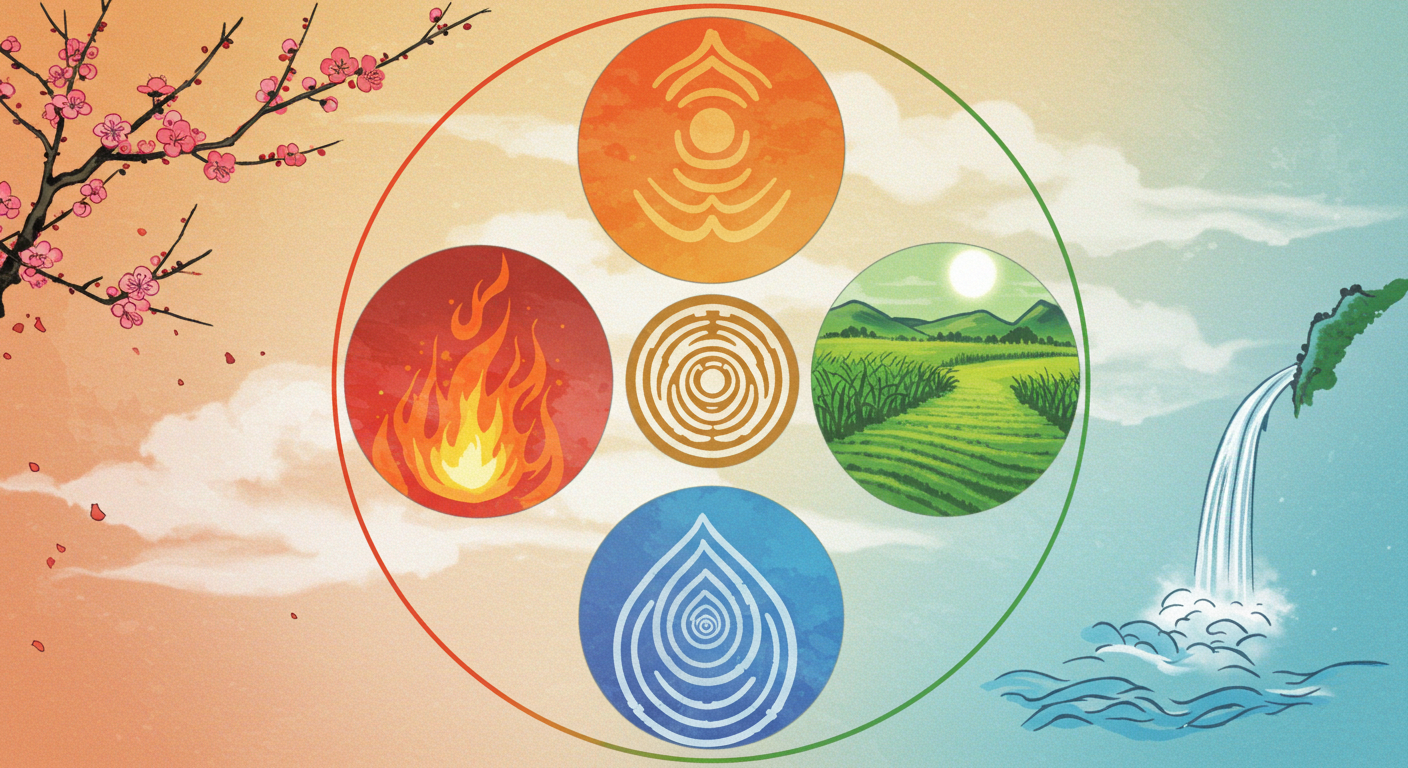
\includegraphics[width=0.85\textwidth]{./images/five-elements.jpg}
\caption{Figure 18: 5 Elements}
\end{figure}

\begin{itemize}
\tightlist
\item
  8 (八): 东,南,西,北,春,夏,秋,冬 (directions and seasons)

  \begin{itemize}
  \tightlist
  \item
    Spatiotemporal 元字
  \item
    Complete system of orientation and cyclical change
  \item
    Foundation for location/directional and time-based concepts
  \end{itemize}
\end{itemize}

\begin{figure}
\centering
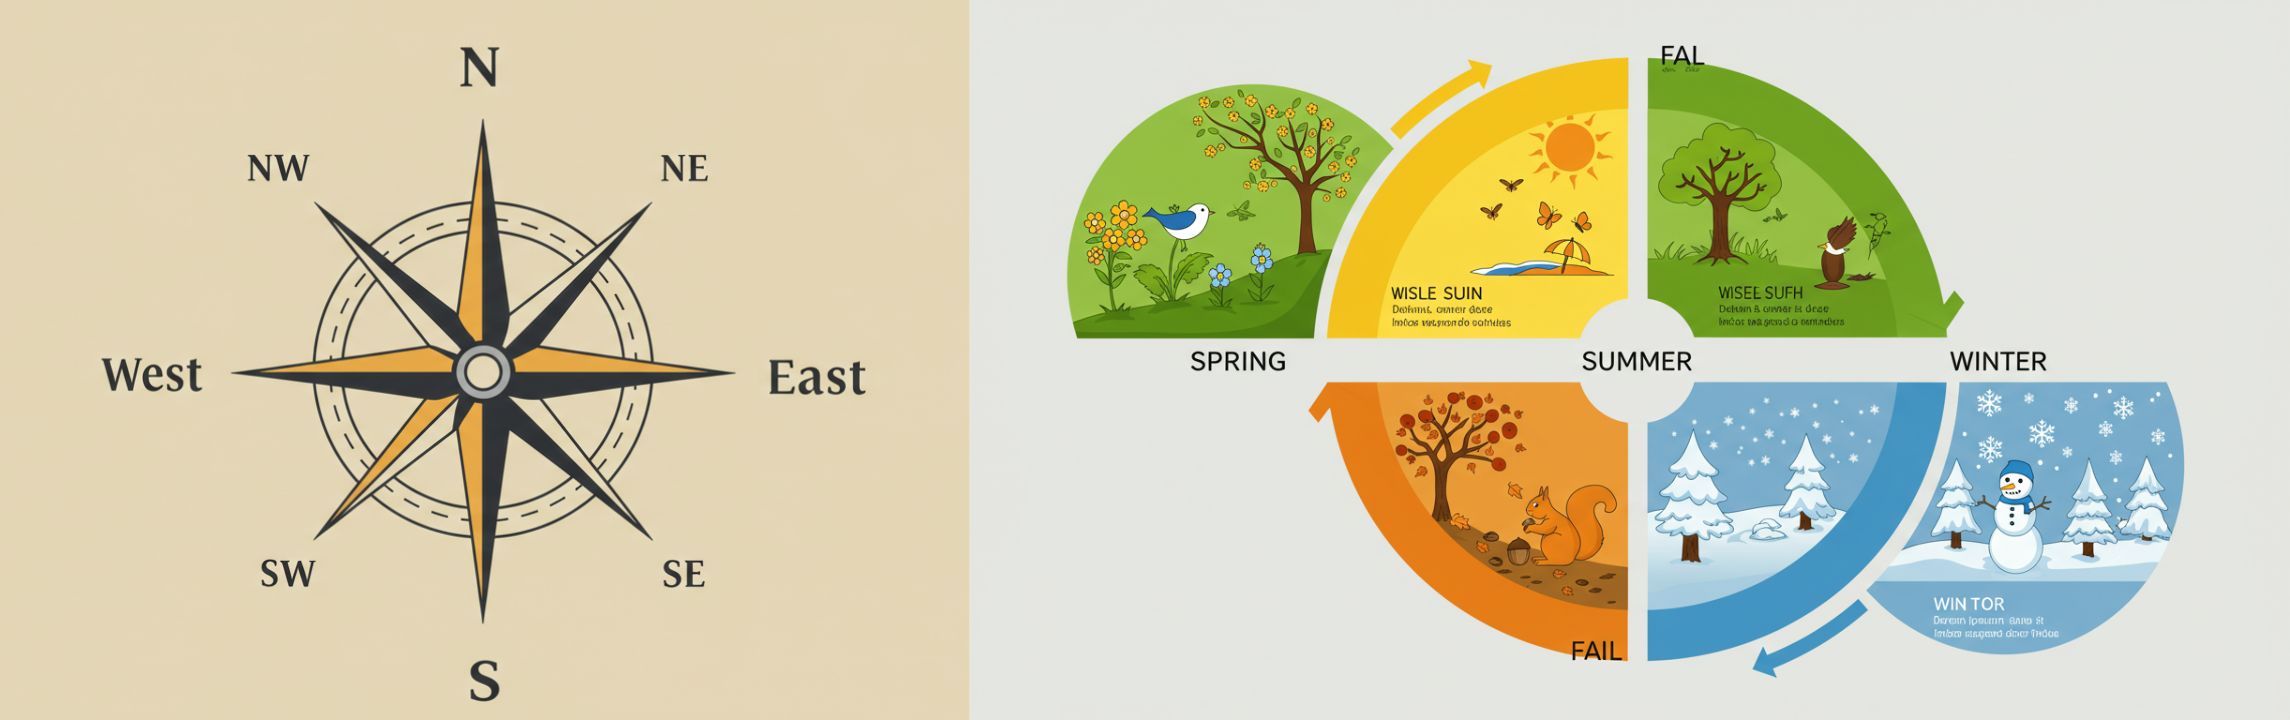
\includegraphics[width=0.85\textwidth]{./images/8-directions-seasons.png}
\caption{Figure 19: 4 Seasons and 8 Directions}
\end{figure}

\begin{itemize}
\tightlist
\item
  13 (十三): 生,鼠,牛,虎,兔,龙,蛇,马,羊,猴,鸡,狗,猪 (basic life forms
  expressed in 12 Zodiac animals)

  \begin{itemize}
  \tightlist
  \item
    Biological object 元字
  \item
    Complex natural phenomena
  \item
    Base set for describing living things
  \item
    Radical form mapping: 牜for 牛, 虫 is a radical for 蛇 and other
    insects, 犭is a radical for many animals (e.g.~猴,狗,猪), 羊,⺶,⺷
    are variant radical forms for 羊(Sheep), radical for 马 appears
    narrower.
  \end{itemize}
\end{itemize}

\begin{figure}
\centering
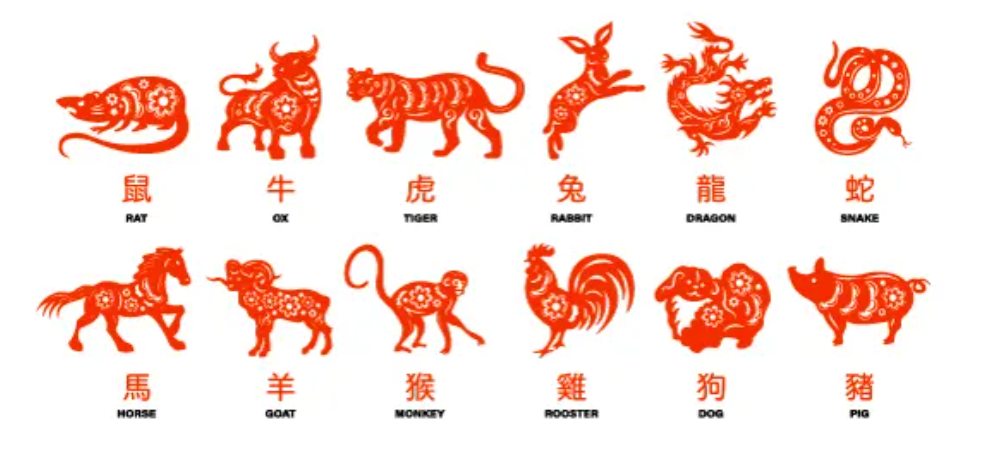
\includegraphics[width=0.85\textwidth]{./images/12-zodiac-animals.png}
\caption{Figure 20: 12 Animals}
\end{figure}

\begin{itemize}
\tightlist
\item
  21 (二十一): Quantification and Measurement 元字

  \begin{itemize}
  \tightlist
  \item
    Numerical System (15 characters):

    \begin{itemize}
    \tightlist
    \item
      Basic numerals: 一 (1),二 (2),三 (3),四 (4),五 (5),六 (6),七
      (7),八 (8),九 (9),十 (10)
    \item
      Large quantities: 百 (100),千 (1000),万 (10,000),亿
      (100,000,000),零 (0)
    \item
      These form the foundation for all quantitative description
    \end{itemize}
  \item
    Physical Units (6 characters):

    \begin{itemize}
    \tightlist
    \item
      Time measurement: 秒 (s),分 (m),时 (h)

      \begin{itemize}
      \tightlist
      \item
        Progression from smallest (second) to largest (hour)
      \item
        Reflects natural cycles and human activity patterns
      \end{itemize}
    \item
      Length measurement: 寸 (cm),丈 (m),里 (km)

      \begin{itemize}
      \tightlist
      \item
        Traditional Chinese units of length
      \item
        Scales from human body reference (寸) to geographic distance
        (里)
      \end{itemize}
    \end{itemize}
  \end{itemize}
\end{itemize}

This set represents the emergence of systematic measurement and
counting.

\begin{figure}
\centering
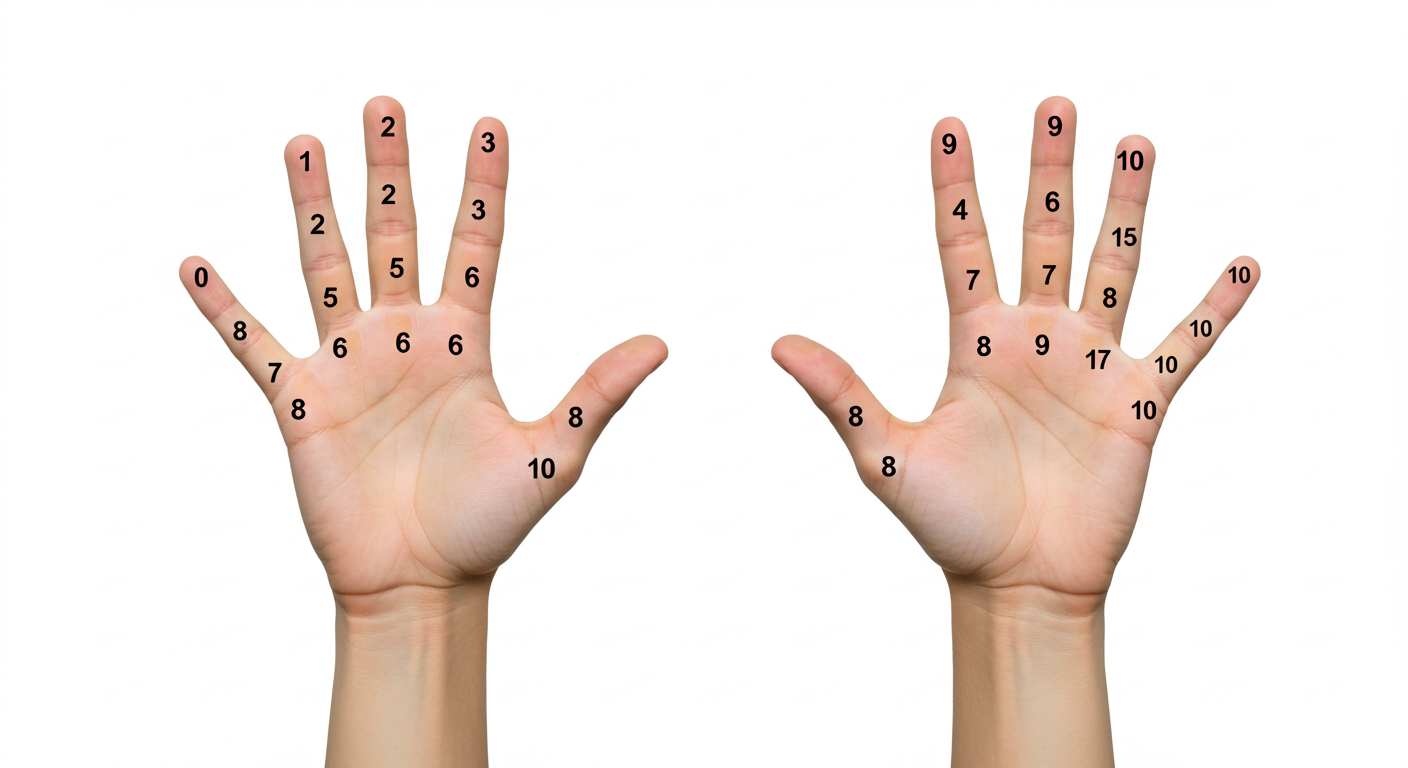
\includegraphics[width=0.85\textwidth]{./images/10-fingers.jpg}
\caption{Figure 21: 10 Fingers}
\end{figure}

\begin{itemize}
\tightlist
\item
  34 (三十四): Human Form and Action 元字

  \begin{itemize}
  \tightlist
  \item
    Basic parts:
    心(忄),头,首,面,口,目,眉,鼻,耳,舌,牙,齿,手(扌),又,足,血,肉,身,尸,骨,皮,毛(彡)
  \item
    Action indicators: 言(讠), 看,听,思,食(饣),走(辶),立
  \item
    Identity: 男,女,子,自,己
  \item
    Radical form mapping: 忄for 心, 扌,又 for 手, 辶 for 足, 讠for 言,
    饣for 食, often (not always) in action context, e.g.~emotional
    thinking, holding, walking, communicating, respectively. 目, 口, 足,
    骨, 耳 appear as radicals too. Some of these characters (like 首,
    面) can function as both nouns (head, face) and measure
    words/classifiers in different contexts.
  \end{itemize}
\end{itemize}

This set introduces fundamental components for describing human
existence and behavior.

\begin{figure}
\centering
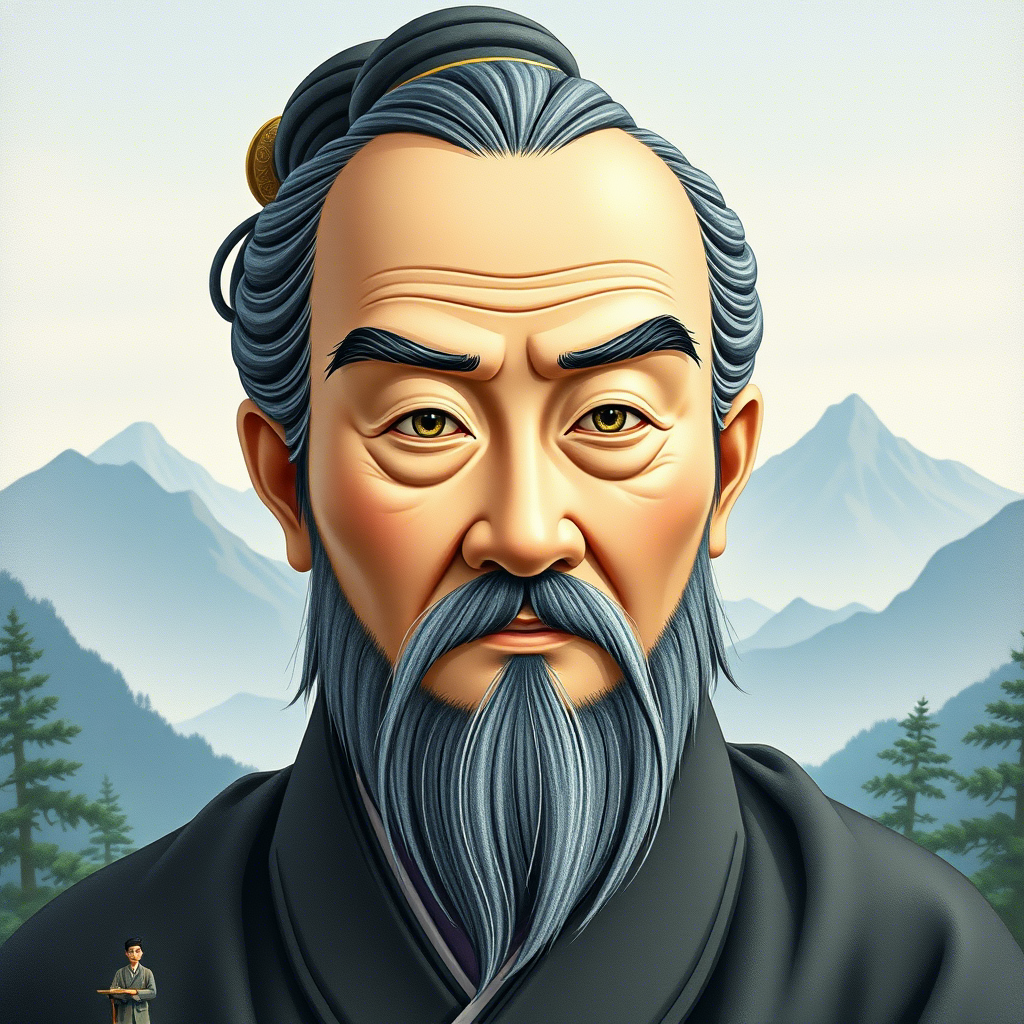
\includegraphics[width=0.85\textwidth]{./images/laozi-qwen-max.png}
\caption{Figure 22: AI generated image of Lao Zi}
\end{figure}

These nine levels demonstrate how Chinese characters evolved naturally
from fundamental concepts to sophisticated human expression, mirroring
the complexity gradients found in natural systems.

\subsubsection{Discussion and
Implications}\label{discussion-and-implications}

\paragraph{4.1 Chinese Writing as a Living
System}\label{chinese-writing-as-a-living-system}

Our computational and physics-inspired analysis reveals Chinese writing
as a living, self-organizing system that mirrors natural growth
patterns. This perspective yields several key insights:

\subparagraph{4.1.1 Emergent Complexity}\label{emergent-complexity}

\begin{itemize}
\tightlist
\item
  Like biological systems emerging from simple molecular interactions,
  complex characters emerge from basic 元字 combinations
\item
  Component relationships evolve naturally based on semantic needs, not
  arbitrary assignments
\item
  New meanings emerge through systematic combination patterns
\item
  Character evolution follows principles similar to natural growth
  patterns seen in Fibonacci sequences
\item
  The progression from basic elements (气, 点, 线) to sophisticated
  human concepts demonstrates organic development
\end{itemize}

\subparagraph{4.1.2 Self-Organization
Principles}\label{self-organization-principles}

\begin{itemize}
\tightlist
\item
  Characters form stable patterns without centralized design
\item
  Component combinations follow natural efficiency principles
\item
  Semantic relationships develop through organic usage patterns
\item
  System exhibits both stability (preserving core meanings) and
  adaptability (generating new combinations)
\item
  Character families demonstrate natural clustering and relationship
  patterns
\end{itemize}

\subparagraph{4.1.3 Adaptive Resilience}\label{adaptive-resilience}

\begin{itemize}
\tightlist
\item
  System maintains coherence while allowing innovation
\item
  Character combinations show remarkable flexibility in expressing new
  concepts
\item
  Ancient elements remain relevant for modern technical terms
\item
  Core semantic foundations support endless expansion
\end{itemize}

\paragraph{4.2 Practical Implications}\label{practical-implications}

\subparagraph{4.2.1 Learning Strategy}\label{learning-strategy}

\begin{itemize}
\tightlist
\item
  Focus on elemental character (元字) and their core concepts
\item
  Reduce the fundamental 元字 set to lower the entry-barrier in learning
  Chinese
\item
  Learn the set of 400 元字 first as foundation
\item
  Recognize systematic structure instead of memorizing thousands of
  individual characters
\item
  Understand natural combination patterns rather than arbitrary
  associations
\end{itemize}

\subparagraph{4.2.2 Educational
Applications}\label{educational-applications}

\begin{itemize}
\tightlist
\item
  Promote concept-based learning across disciplines
\item
  Break down artificial barriers between language, mathematics, and
  science
\item
  Make STEM-oriented learning accessible to earlier ages through
  character analysis
\item
  Use character evolution to teach systematic thinking
\item
  Leverage natural patterns to enhance memorization and understanding
\end{itemize}

\subparagraph{4.2.3 Modern Applications}\label{modern-applications}

\begin{itemize}
\tightlist
\item
  Character design principles for digital fonts
\item
  Input method optimization based on component patterns
\item
  Natural language processing models based on character component
  relationships
\item
  AI applications in character recognition and generation
\item
  Development of new technical terminology
\item
  Cross-cultural communication of scientific concepts
\end{itemize}

\paragraph{4.3 Basic Research in Other Natural
Languages}\label{basic-research-in-other-natural-languages}

The methodologies and insights developed in this analysis of Chinese
characters suggest promising directions for studying other natural
languages:

\subparagraph{4.3.1 Computational
Approaches}\label{computational-approaches}

\begin{itemize}
\tightlist
\item
  Apply network analysis to study semantic relationships and word
  formation patterns
\item
  Investigate natural clustering and organizational principles in
  vocabulary
\item
  Analyze language evolution through computational models
\item
  Map concept hierarchies across different languages
\end{itemize}

\subparagraph{4.3.2 Physics-Inspired
Analysis}\label{physics-inspired-analysis}

\begin{itemize}
\tightlist
\item
  Use reductionist approaches to identify fundamental linguistic
  elements
\item
  Study language as a complex adaptive system
\item
  Apply principles of self-organization to understand language evolution
\item
  Investigate universal patterns in language structure
\end{itemize}

\subparagraph{4.3.3 Enhanced Learning
Frameworks}\label{enhanced-learning-frameworks}

\begin{itemize}
\tightlist
\item
  Simplify language learning by identifying core patterns and elements
\item
  Create concept-based learning approaches that transcend specific
  languages
\item
  Develop multi-modal learning experiences that leverage natural
  associations
\item
  Build cross-linguistic bridges through shared conceptual foundations
\end{itemize}

\subparagraph{4.3.4 AI-Enhanced
Applications}\label{ai-enhanced-applications}

\begin{itemize}
\tightlist
\item
  Leverage AI for personalized, multi-lingual learning experiences
\item
  Create interactive visualizations of language relationships
\item
  Develop tools for concept-based cross-language translation
\item
  Enable dynamic, context-aware language learning environments
\end{itemize}

This analysis suggests that viewing languages as living, evolving
systems rather than fixed sets of rules opens new possibilities for
learning, teaching, and research. The natural principles revealed in
Chinese character formation and evolution can inform both theoretical
understanding and practical applications across multiple languages and
disciplines.

\subsection{Conclusion}\label{conclusion}

This research demonstrates how simplification and deeper understanding
can work hand in hand in the study of Chinese characters. By identifying
422 elemental characters (元字) through computational network analysis,
we have achieved significant simplification of the learning challenge -
reducing the initial memorization burden from thousands of characters to
a manageable set of foundational elements. However, this simplification
leads not to reduction but to enrichment of understanding in several key
ways:

\begin{enumerate}
\def\labelenumi{\arabic{enumi}.}
\tightlist
\item
  From Memorization to Understanding
\end{enumerate}

\begin{itemize}
\tightlist
\item
  Instead of rote learning of thousands of isolated characters
\item
  Learners grasp systematic patterns of character formation
\item
  Understanding how complex meanings emerge from simple elements
\item
  Recognition of natural organizational principles in language
\end{itemize}

\begin{enumerate}
\def\labelenumi{\arabic{enumi}.}
\setcounter{enumi}{1}
\tightlist
\item
  From Static to Dynamic Understanding
\end{enumerate}

\begin{itemize}
\tightlist
\item
  Characters revealed as a living, evolving system
\item
  Clear visualization of how meanings extend from concrete to abstract
\item
  Appreciation of the system's adaptive capacity for new concepts
\item
  Recognition of internal logic in character evolution
\end{itemize}

\begin{enumerate}
\def\labelenumi{\arabic{enumi}.}
\setcounter{enumi}{2}
\tightlist
\item
  From Fragmented to Integrated Knowledge
\end{enumerate}

\begin{itemize}
\tightlist
\item
  Connection between language and natural patterns
\item
  Integration of linguistic, philosophical, and scientific insights
\item
  Bridge between traditional wisdom and modern analysis
\item
  Cross-disciplinary understanding of knowledge organization
\end{itemize}

\begin{enumerate}
\def\labelenumi{\arabic{enumi}.}
\setcounter{enumi}{3}
\tightlist
\item
  From Surface to Deep Structure
\end{enumerate}

\begin{itemize}
\tightlist
\item
  Beyond simple visual components to semantic networks
\item
  Recognition of sophisticated metaphorical thinking
\item
  Understanding of systematic meaning extension
\item
  Appreciation of cultural and cognitive patterns
\end{itemize}

This deeper understanding enriches learning experiences by: - Making
character learning more intuitive and systematic - Revealing connections
across different knowledge domains - Enabling appreciation of cultural
and philosophical dimensions - Supporting creative engagement with the
writing system

The research demonstrates that true simplification comes not from
reduction alone, but from revealing underlying patterns and principles.
By understanding Chinese characters as a naturally evolved system, we
gain both practical advantages in learning and deeper insights into how
human cognition organizes and transmits knowledge. This approach opens
new possibilities for: - AI-enhanced learning tools based on natural
patterns - Cross-cultural communication of complex concepts -
Integration of traditional wisdom with modern analysis - Development of
more intuitive teaching methods

The success of this analysis suggests that the path from simplification
to deeper understanding is not a trade-off but a synergy, where reduced
complexity reveals deeper patterns and richer meanings. This insight has
implications not only for Chinese language learning but for how we
approach the study of complex systems in general.

\subsection{Dedication}\label{dedication}

This work is dedicated to late Professor T.D. Lee(李政道), whose
pioneering efforts opened doors for many Chinese students to pursue
studies and research in the United States, fostering a bridge between
Eastern and Western scientific traditions. His vision and support have
enabled countless scholars like myself to contribute to global
scientific discourse.

This work is also dedicated to author's parents (龚永权,文国芳), who
nurtured his intellectual curiosity through hardships and challenging
times. Their sacrifices and unwavering support are forever remembered.

\subsection{Acknowledgements}\label{acknowledgements}

This paper represents a collaborative effort between the author, and a
team of AI assistants including Claude 3.3 from Anthropic
{[}10{]}, Gemini 2 from Google {[}11{]},
Qwen2.5-Max from Alibaba {[}r\12{]}. The fusion of human
knowledge and insight in software development, physics, and Chinese
language with AI's analytical capabilities enabled the development of
the novel perspectives and methodologies presented in this work. This
collaboration demonstrates the potential of human-AI partnerships in
research and learning, particularly in interdisciplinary studies
bridging traditional knowledge with modern computational technologies.

\subsection{References}\label{references}

{[}1{]} https://www.wikiwand.com/en/articles/Chinese\_characters

{[}2{]} 說文解字 : https://www.shuowen.org/

{[}3{]} Sears, Richard. Chinese Etymology research website at
https://hanziyuan.net/

{[}4{]} Kangxi radicals :
https://en.wikipedia.org/wiki/Kangxi\_radicals


{[}5{]} CC-CEDICT dictionary dataset :
https://www.mdbg.net/chinese/dictionary?page=cc-cedict

{[}6{]} 书同文 汉字网 HSK 汉语水平考试汉字列表 :
https://hanzi.unihan.com.cn/School/HSK

{[}7{]} 漢語拆字字典 : https://github.com/kfcd/chaizi

{[}8{]}
https://www.wikiwand.com/en/articles/Fibonacci\_sequence

{[}9{]} Google ImageFx text-to-image generation tool:
https://labs.google/fx/tools/image-fx

{[}10{]} Claude AI : https://claude.ai/

{[}11{]} Gemini 2.0 : https://gemini.google.com/app

{[}r\12{]} Qwen2.5-MAX : https://chat.qwenlm.ai/


\end{document}